\chapter{Specific Requirements}

\section{External Interface Requirements}

\subsection{User Interfaces}

% screenshots here
\begin{figure}[H]
	\centering     %%% not \center
	\subfigure[Log In page.]{\label{fig:a}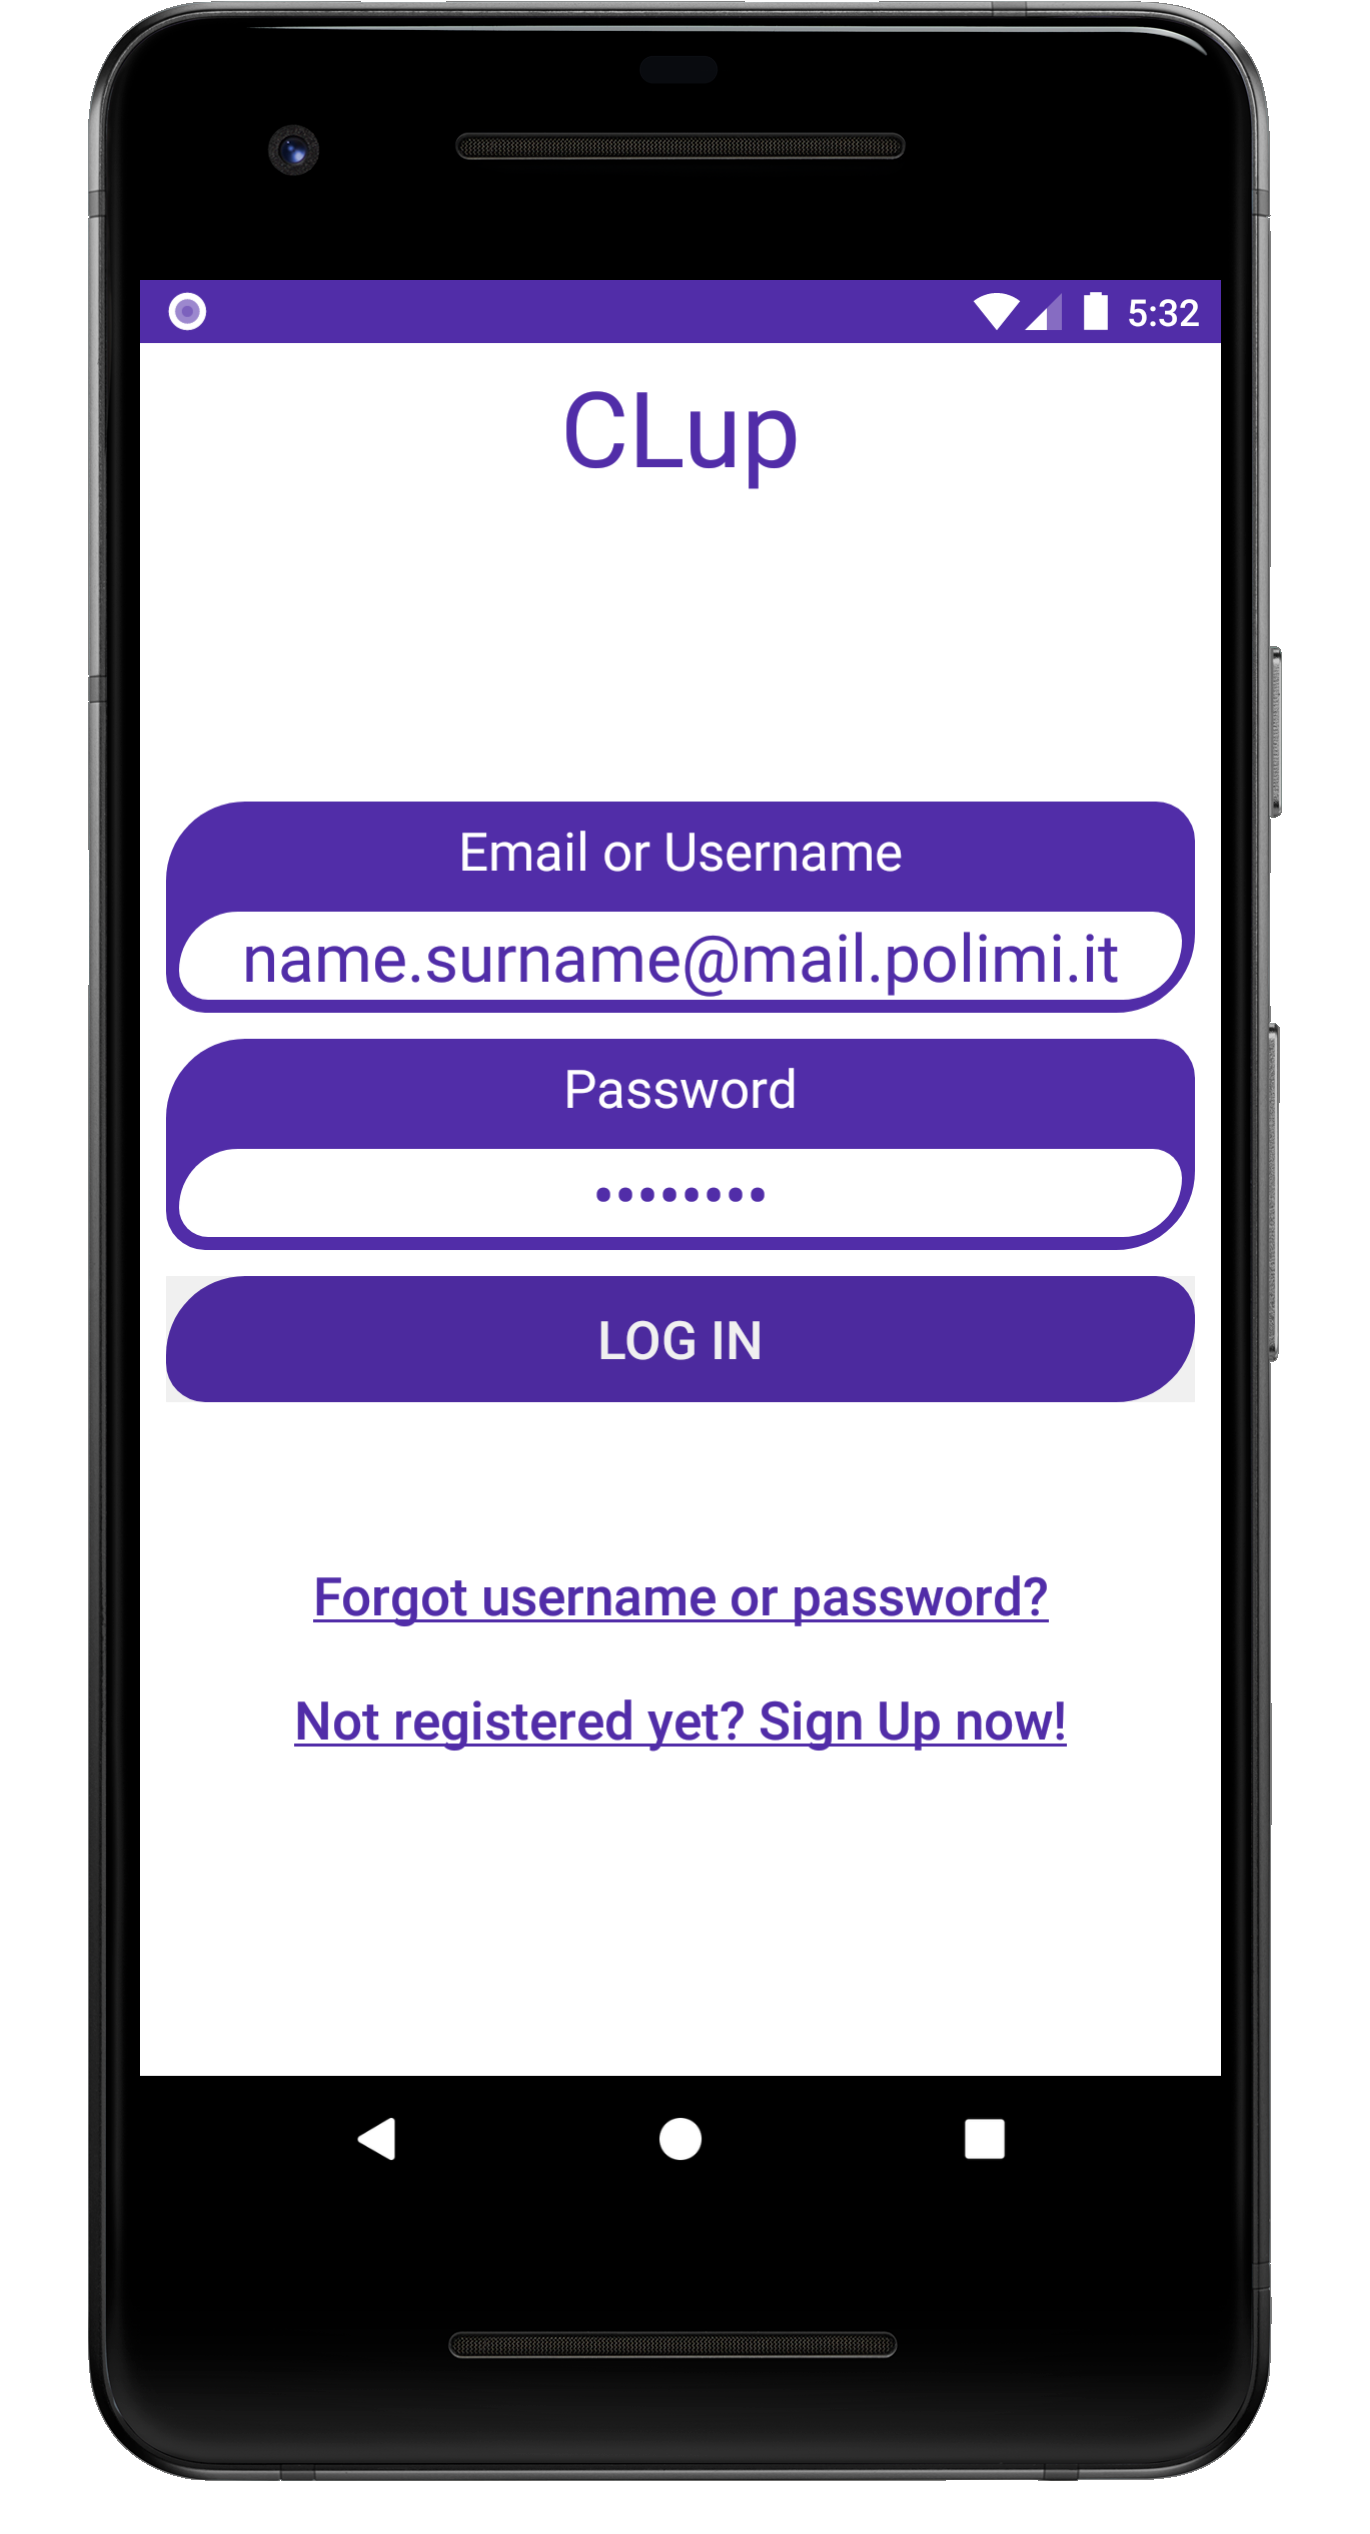
\includegraphics[width=0.4\textwidth]{images/log_in.png}}
	\subfigure[Sign Up page.]{\label{fig:b}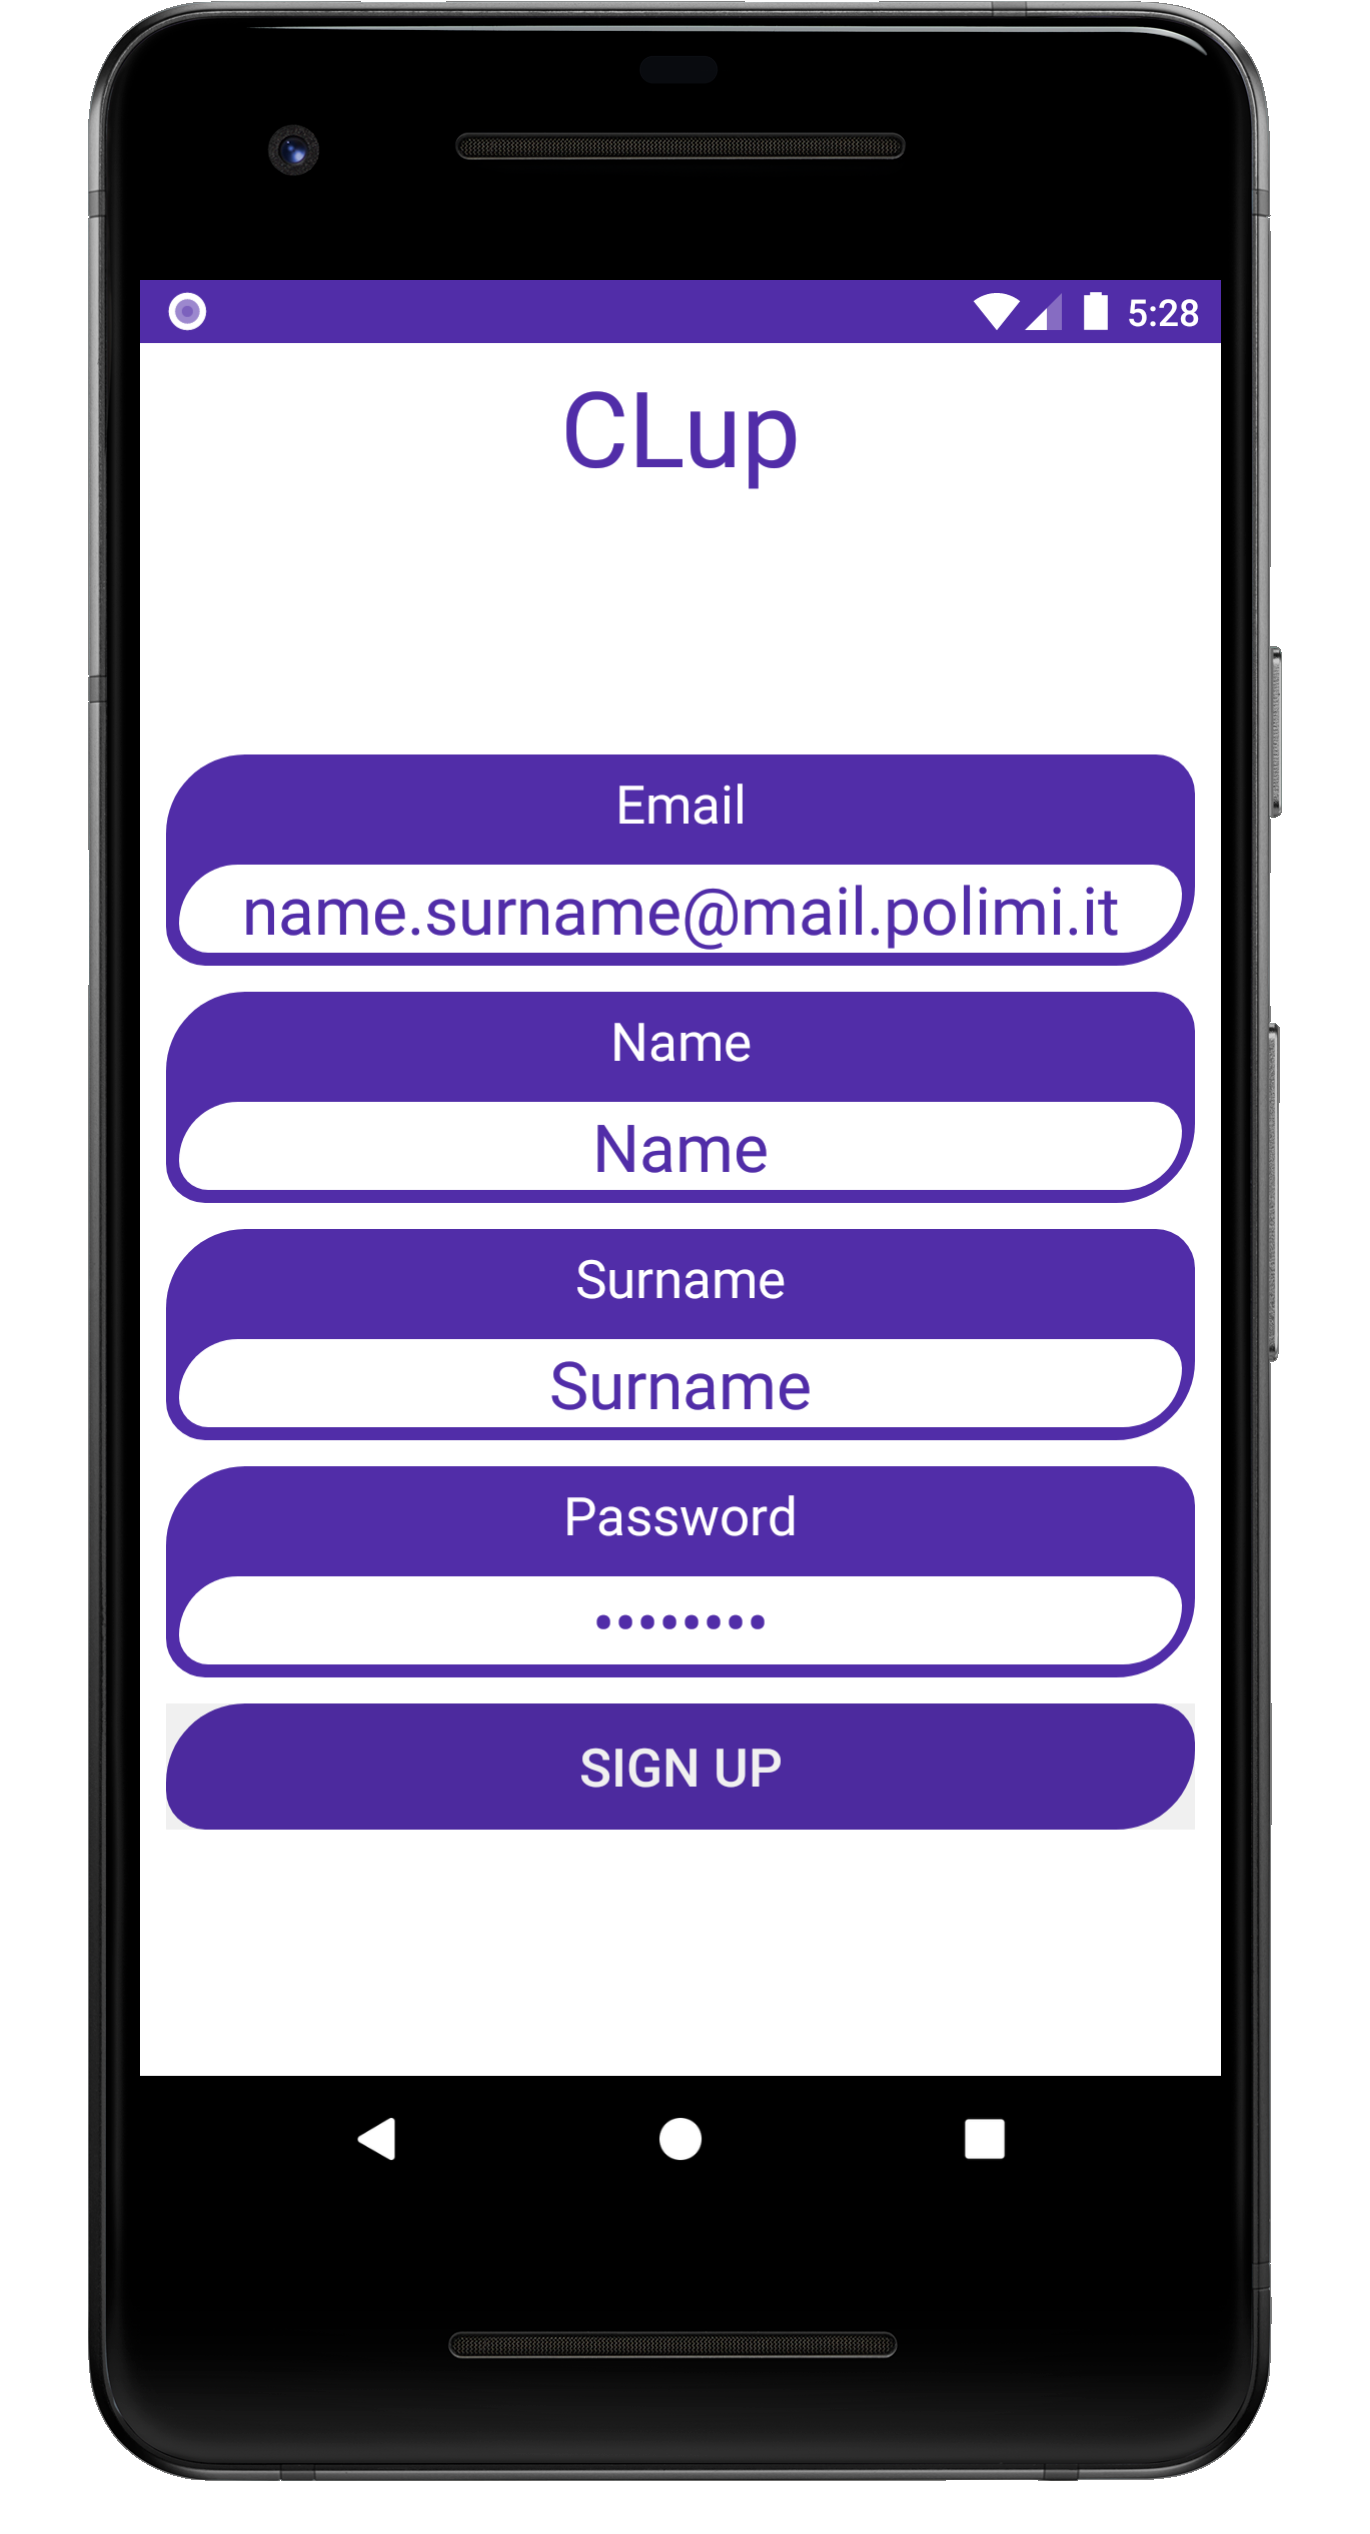
\includegraphics[width=0.4\textwidth]{images/sign_up.png}}
	\caption{Example of Log In and Sign Up pages.}
\end{figure}

\begin{figure}[H]
	\centering
	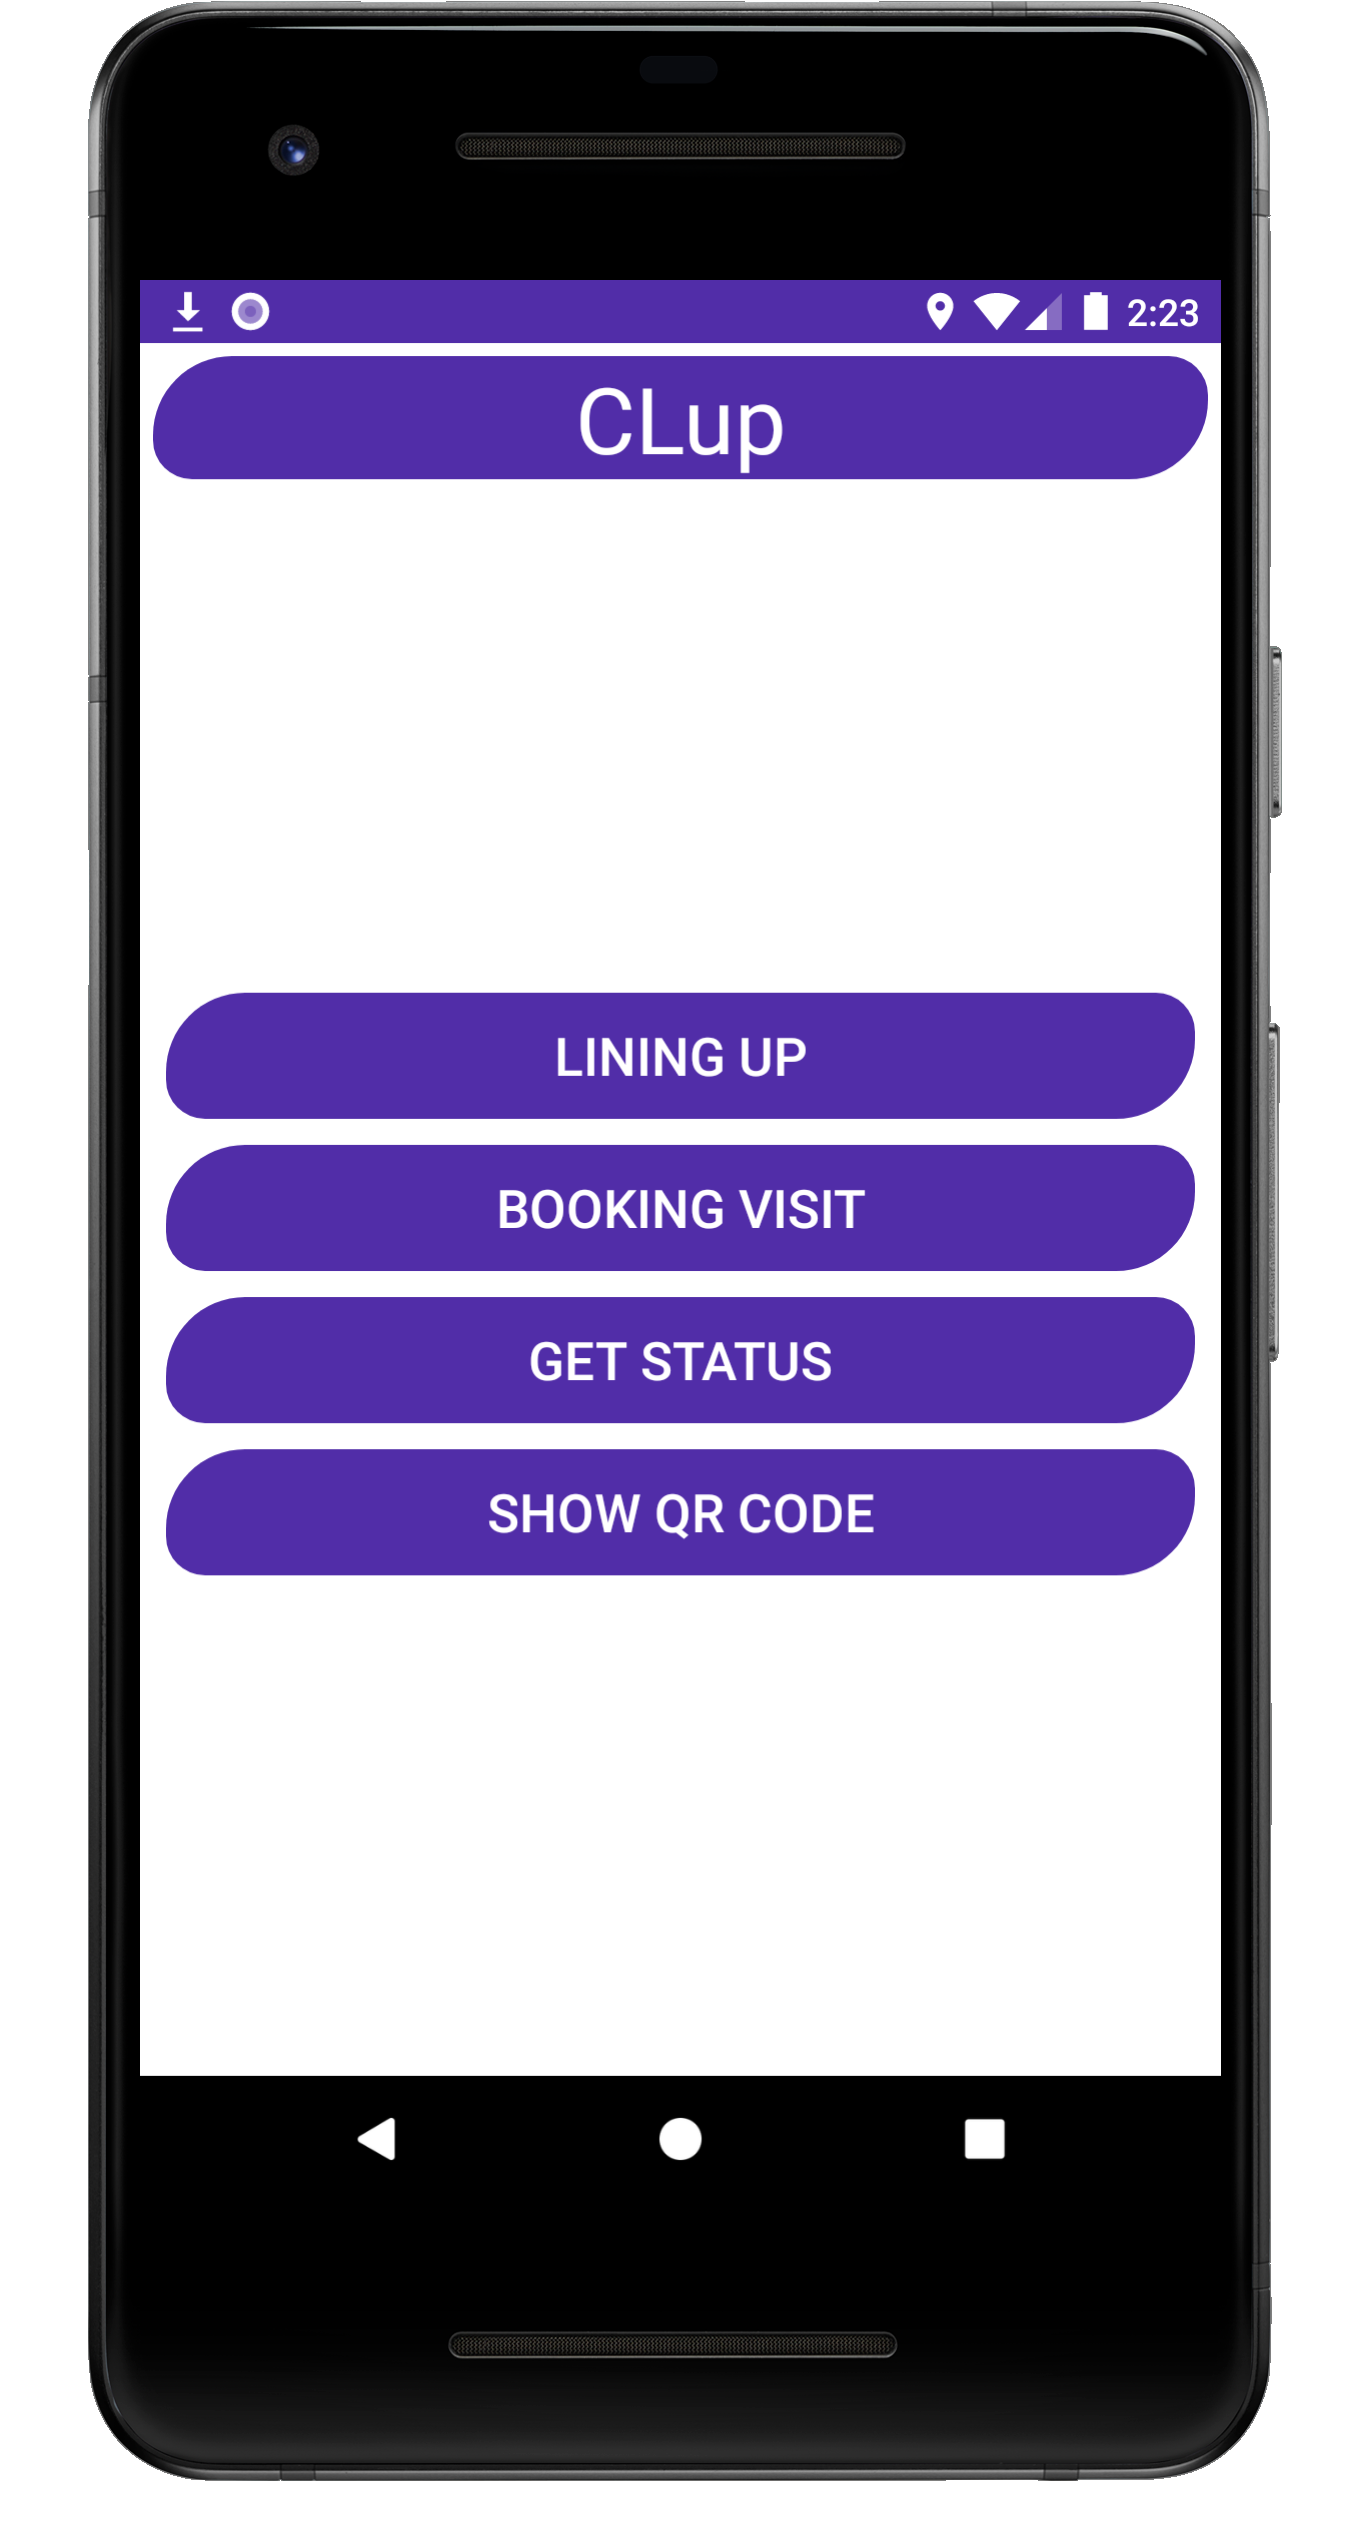
\includegraphics[width=0.35\textwidth]{images/home.png}
	\caption{Home page.}
	\label{customersUseCasesDiagram}
\end{figure}

\begin{figure}[H]
	\centering     %%% not \center
	\subfigure[Lining Up page.]{\label{fig:a}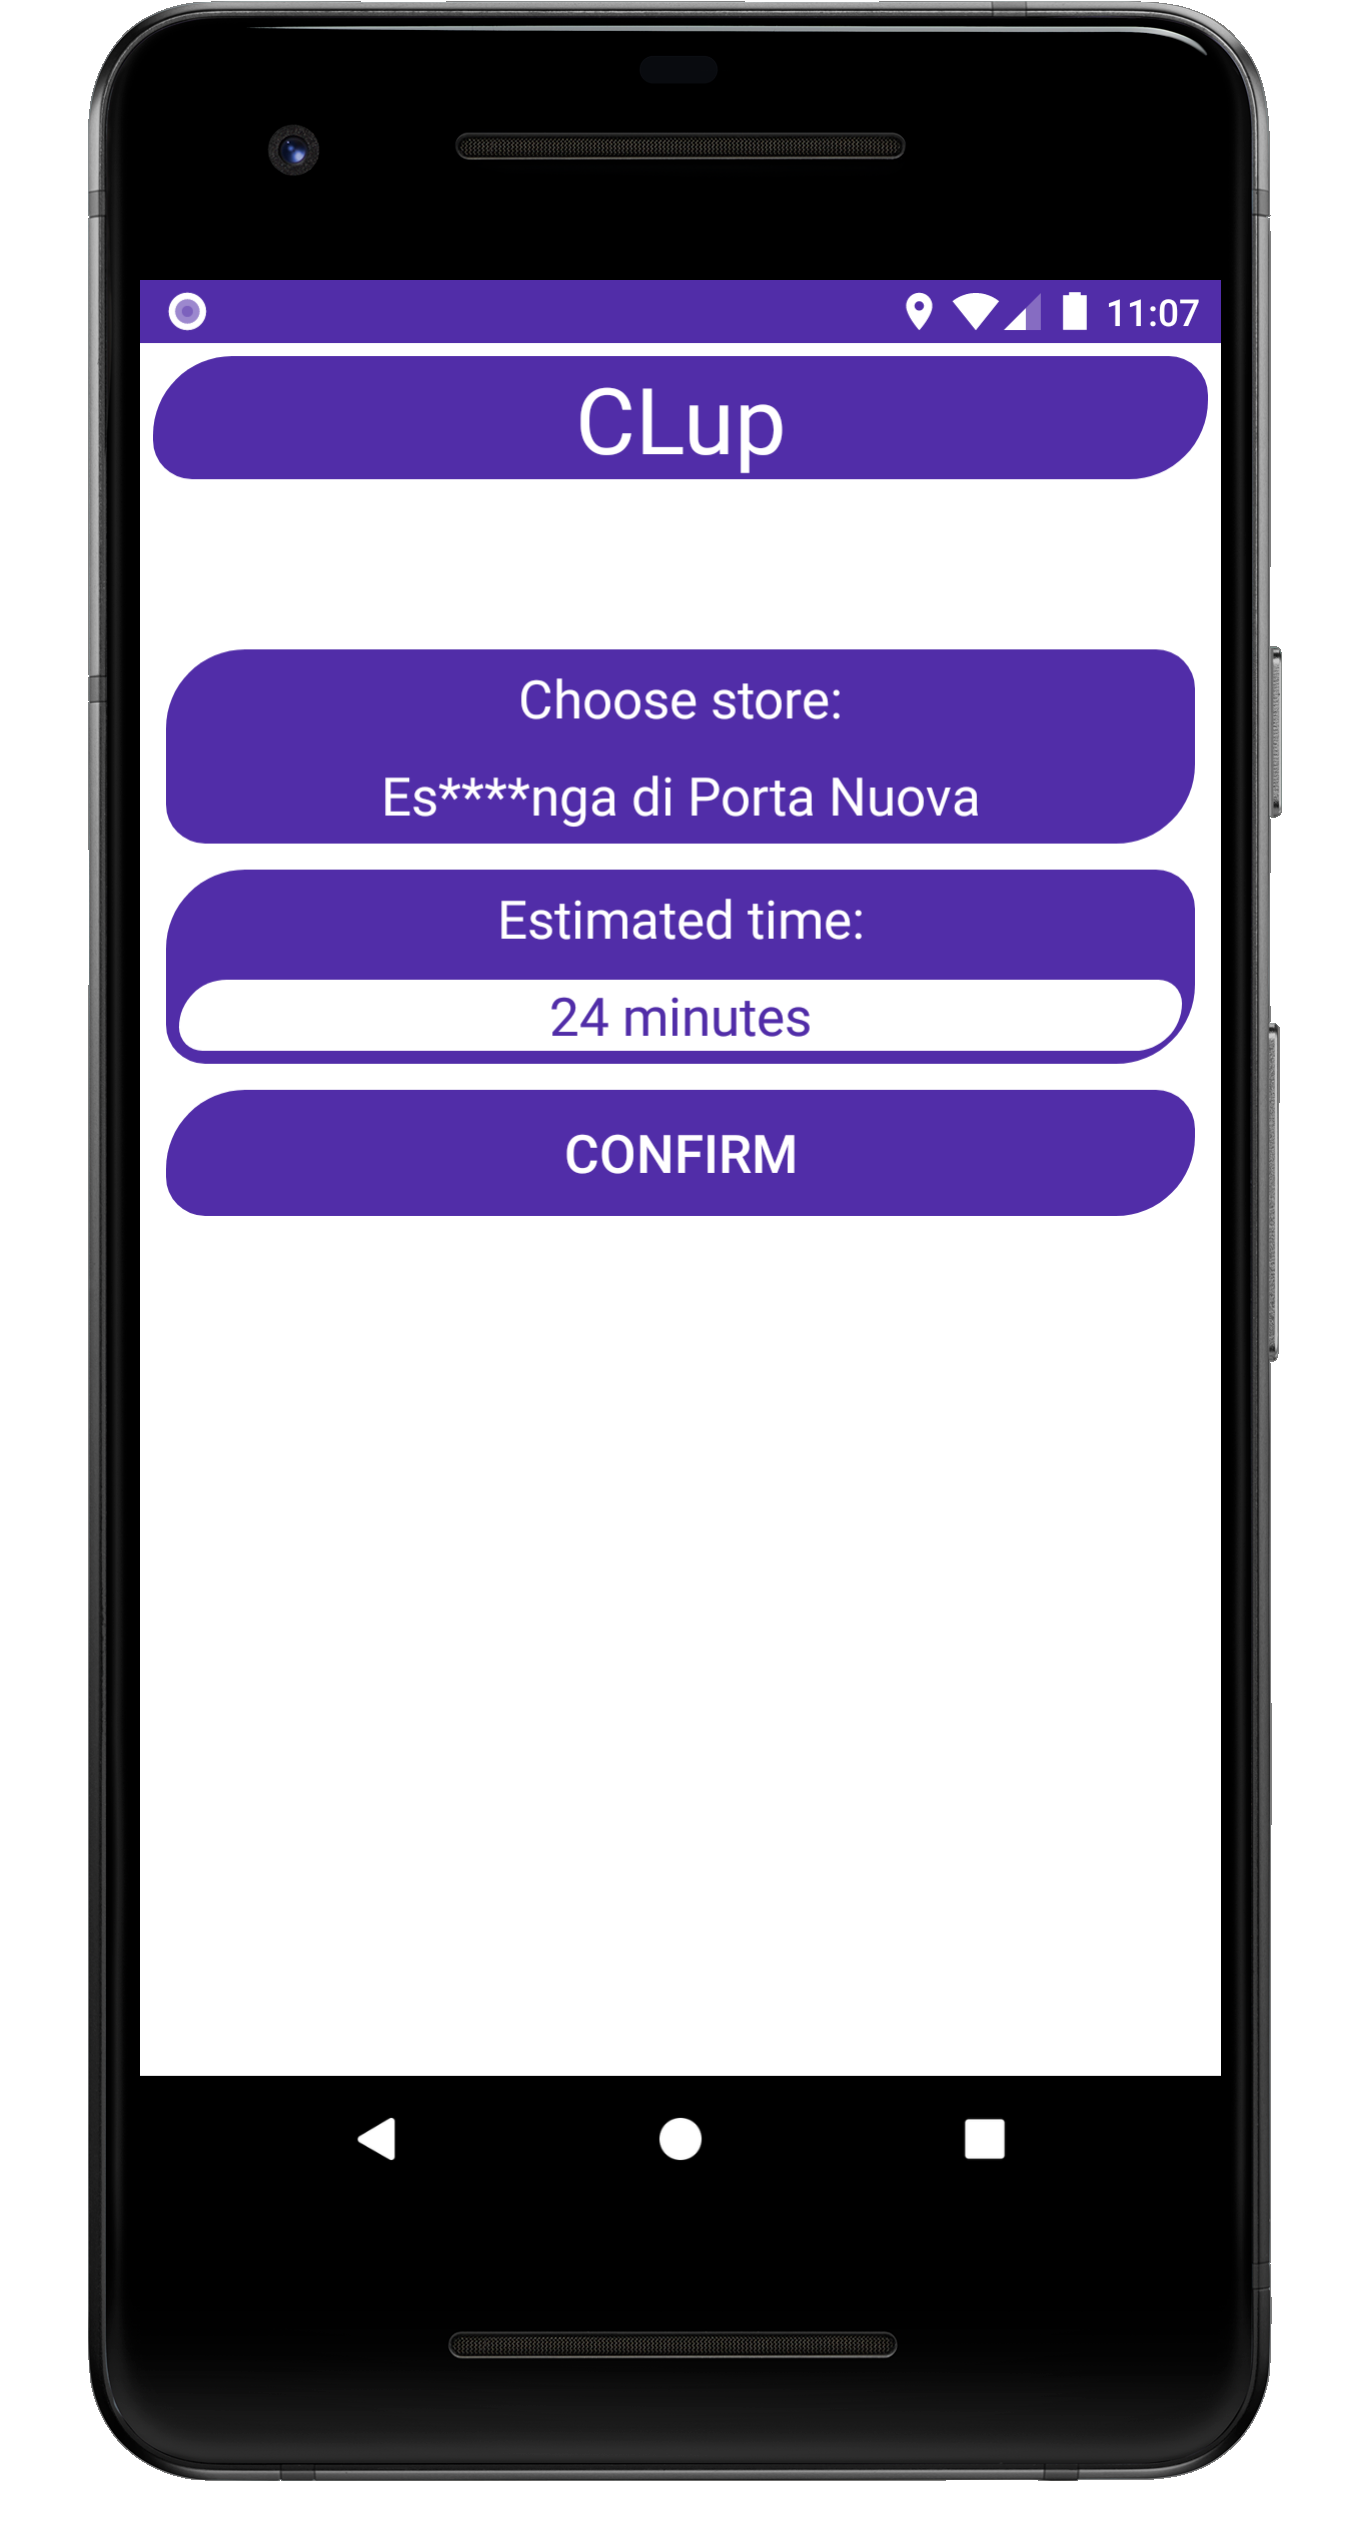
\includegraphics[width=0.4\textwidth]{images/lining_up_01.png}}
	\subfigure[Booking Visit page.]{\label{fig:b}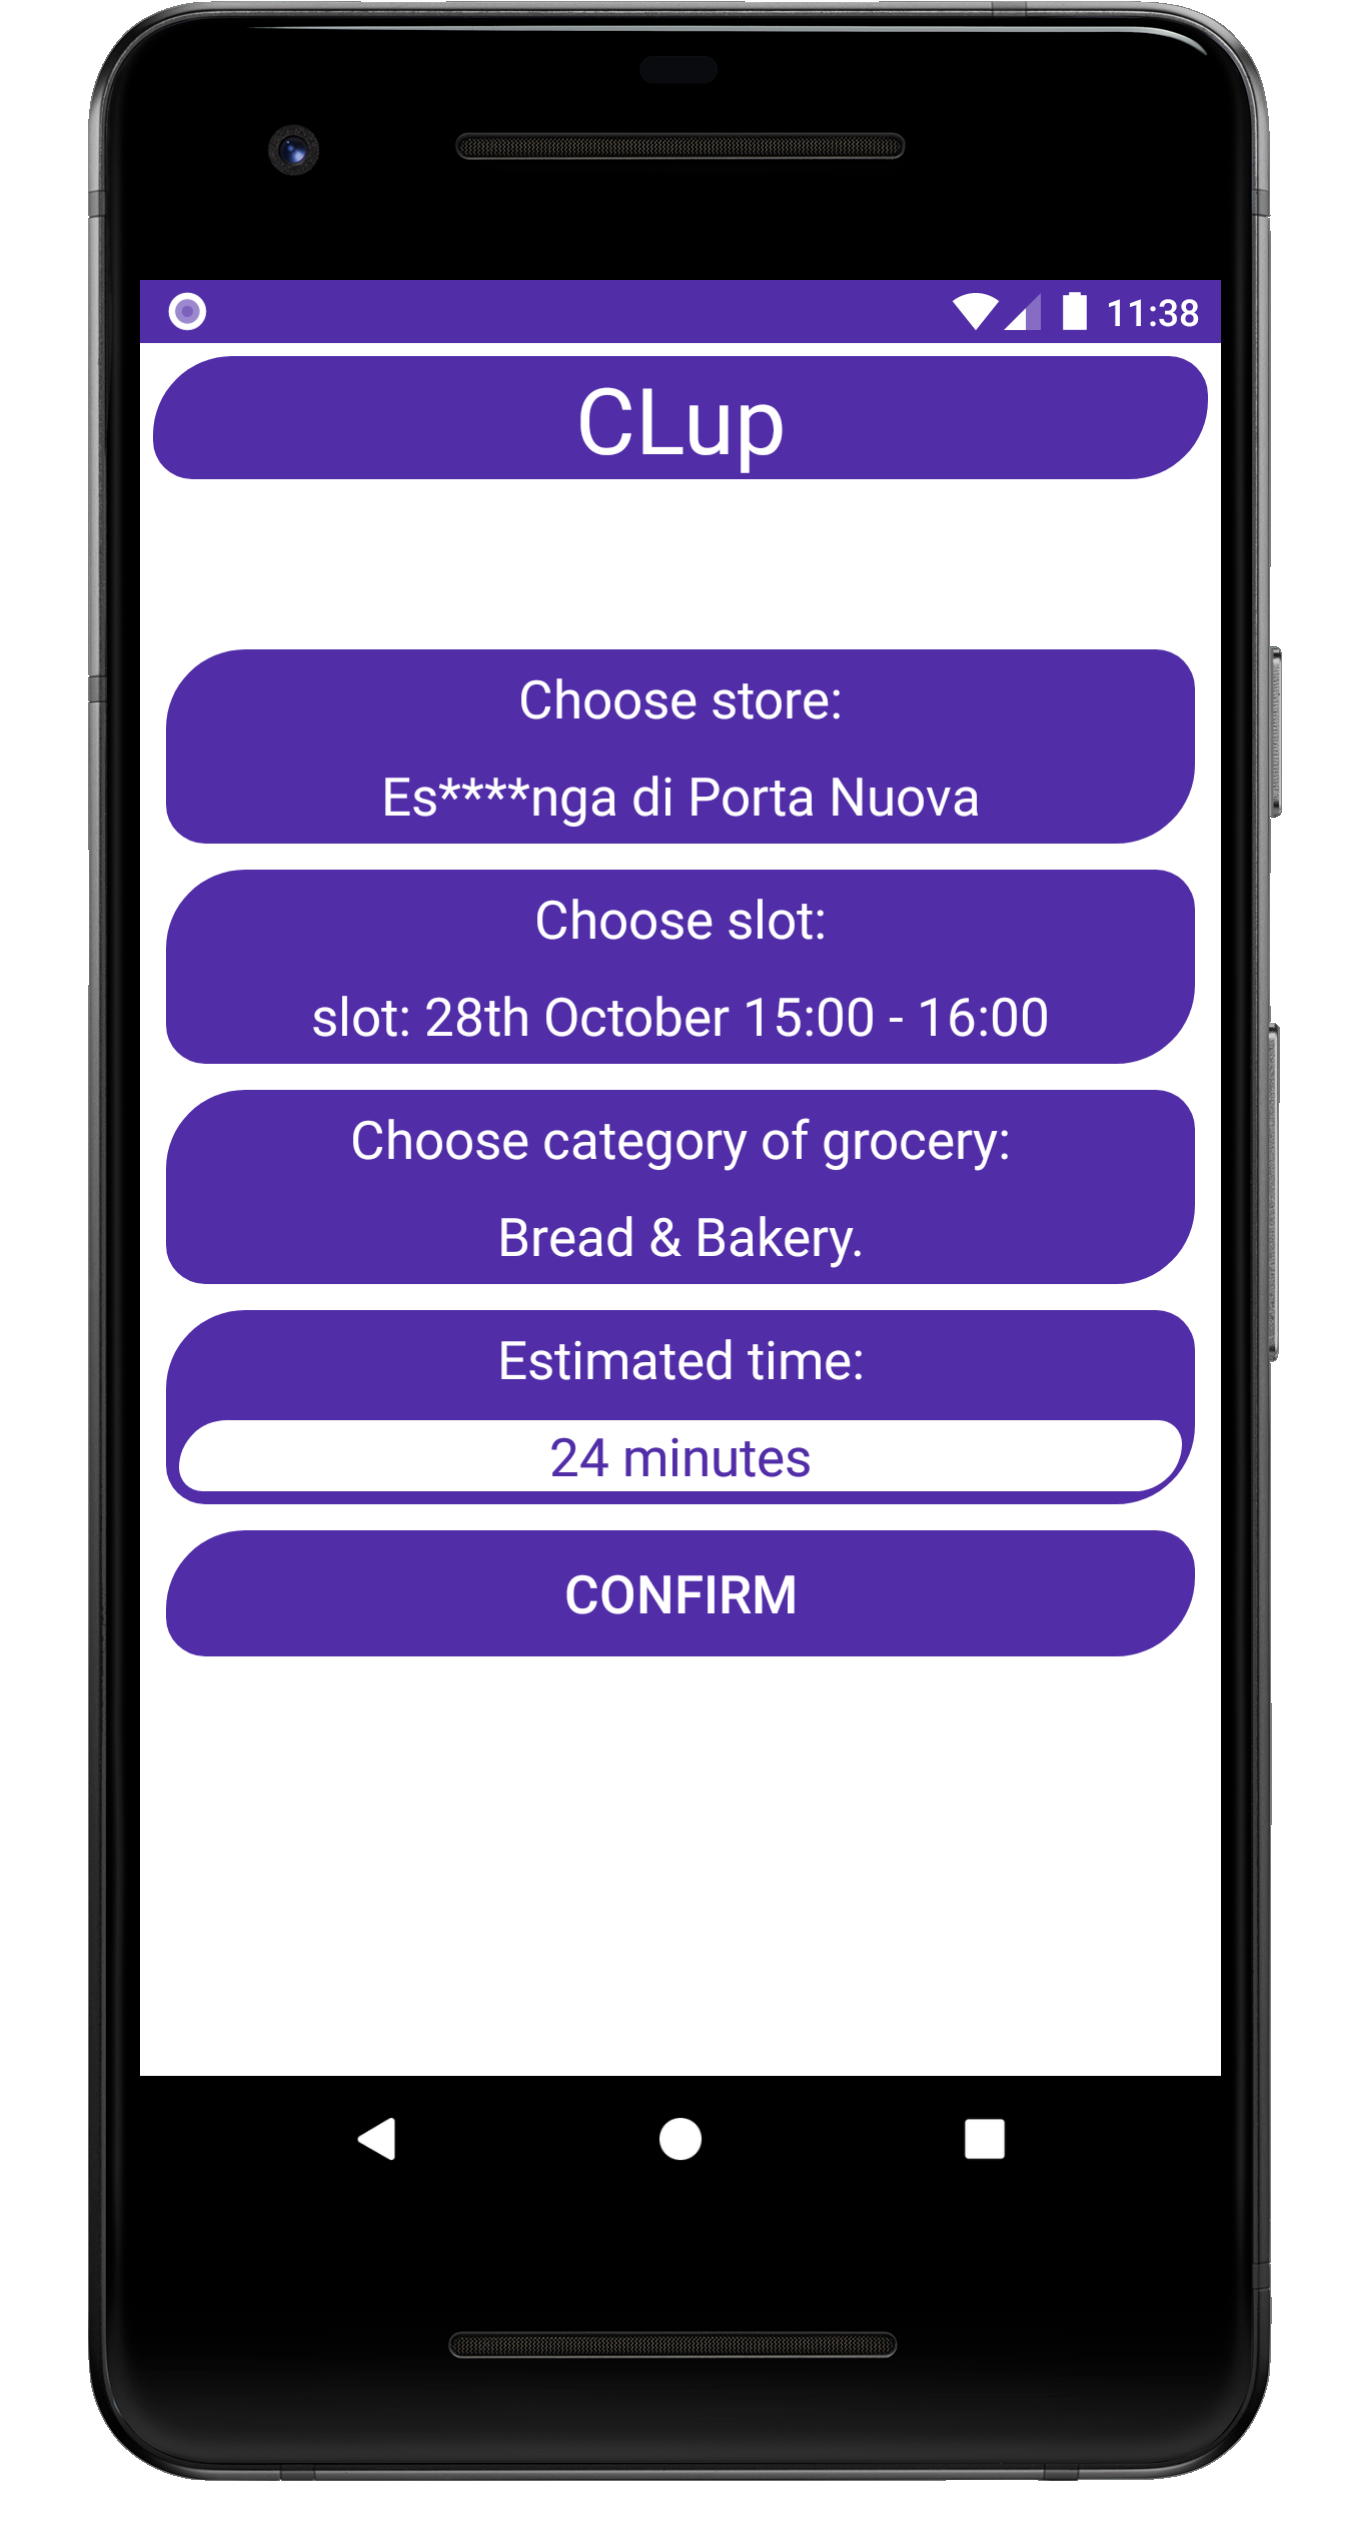
\includegraphics[width=0.4\textwidth]{images/booking_visit_01.png}}
	
	\subfigure[Lining Up page with expanded spinner.]{\label{fig:c}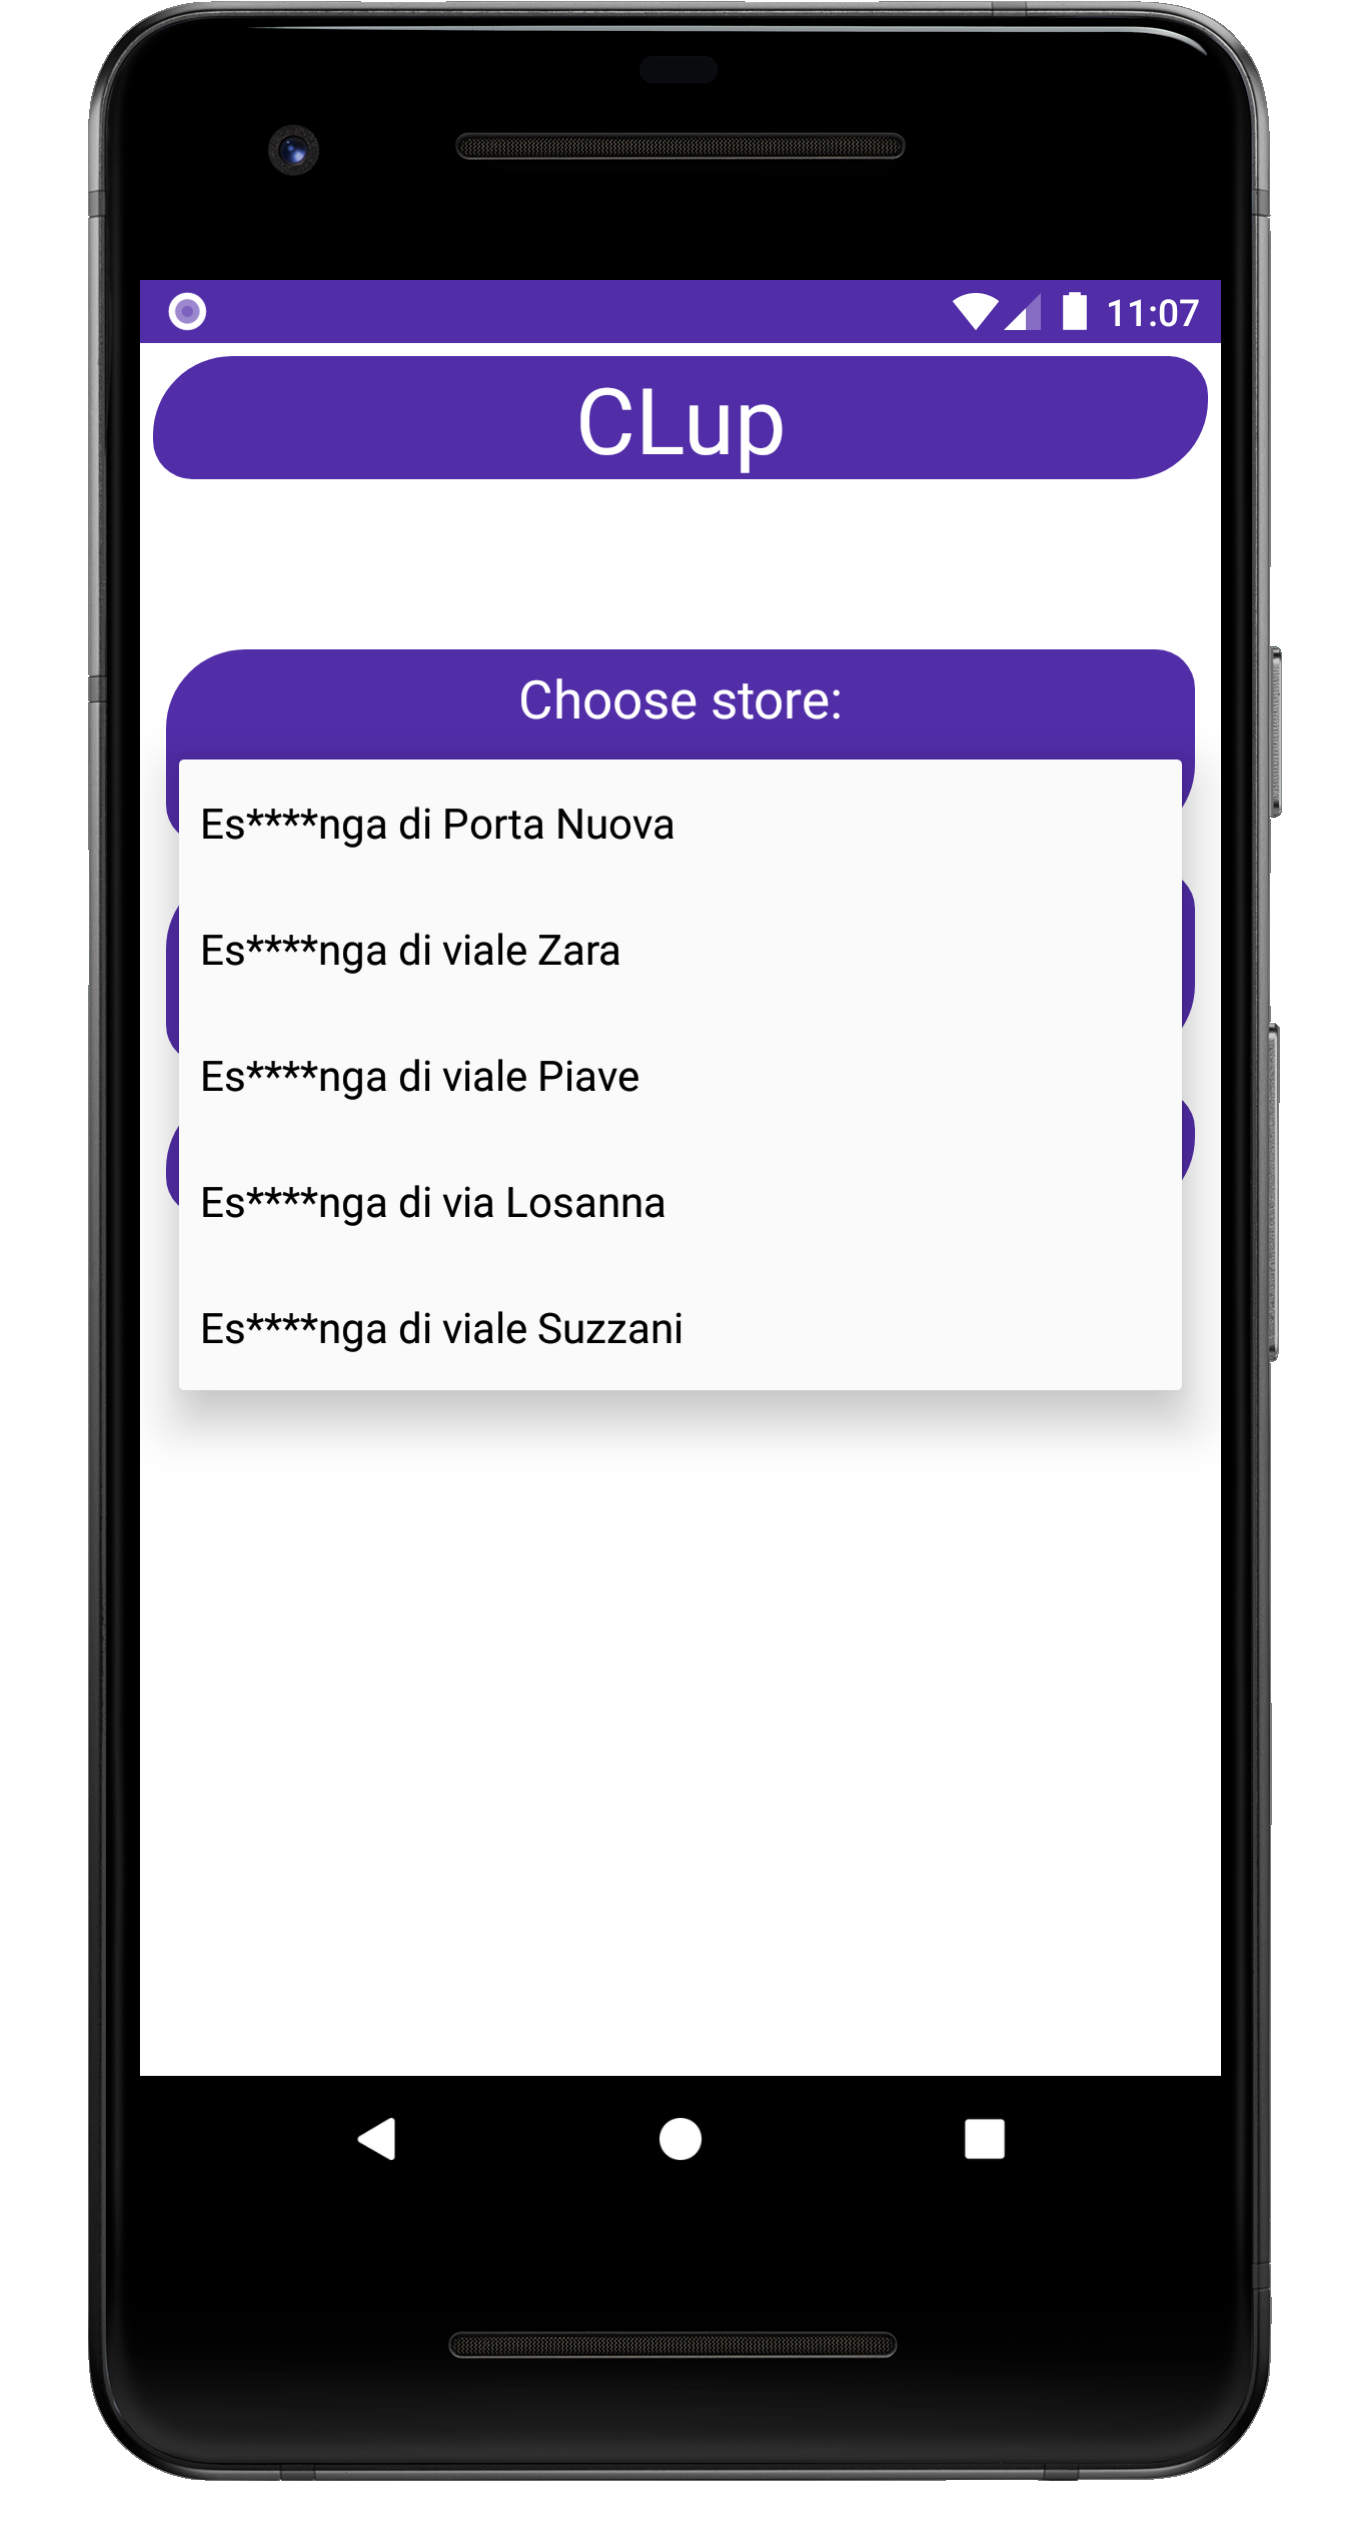
\includegraphics[width=0.4\textwidth]{images/lining_up_02.png}}
	\subfigure[Booking Visit page with expanded spinner.]{\label{fig:d}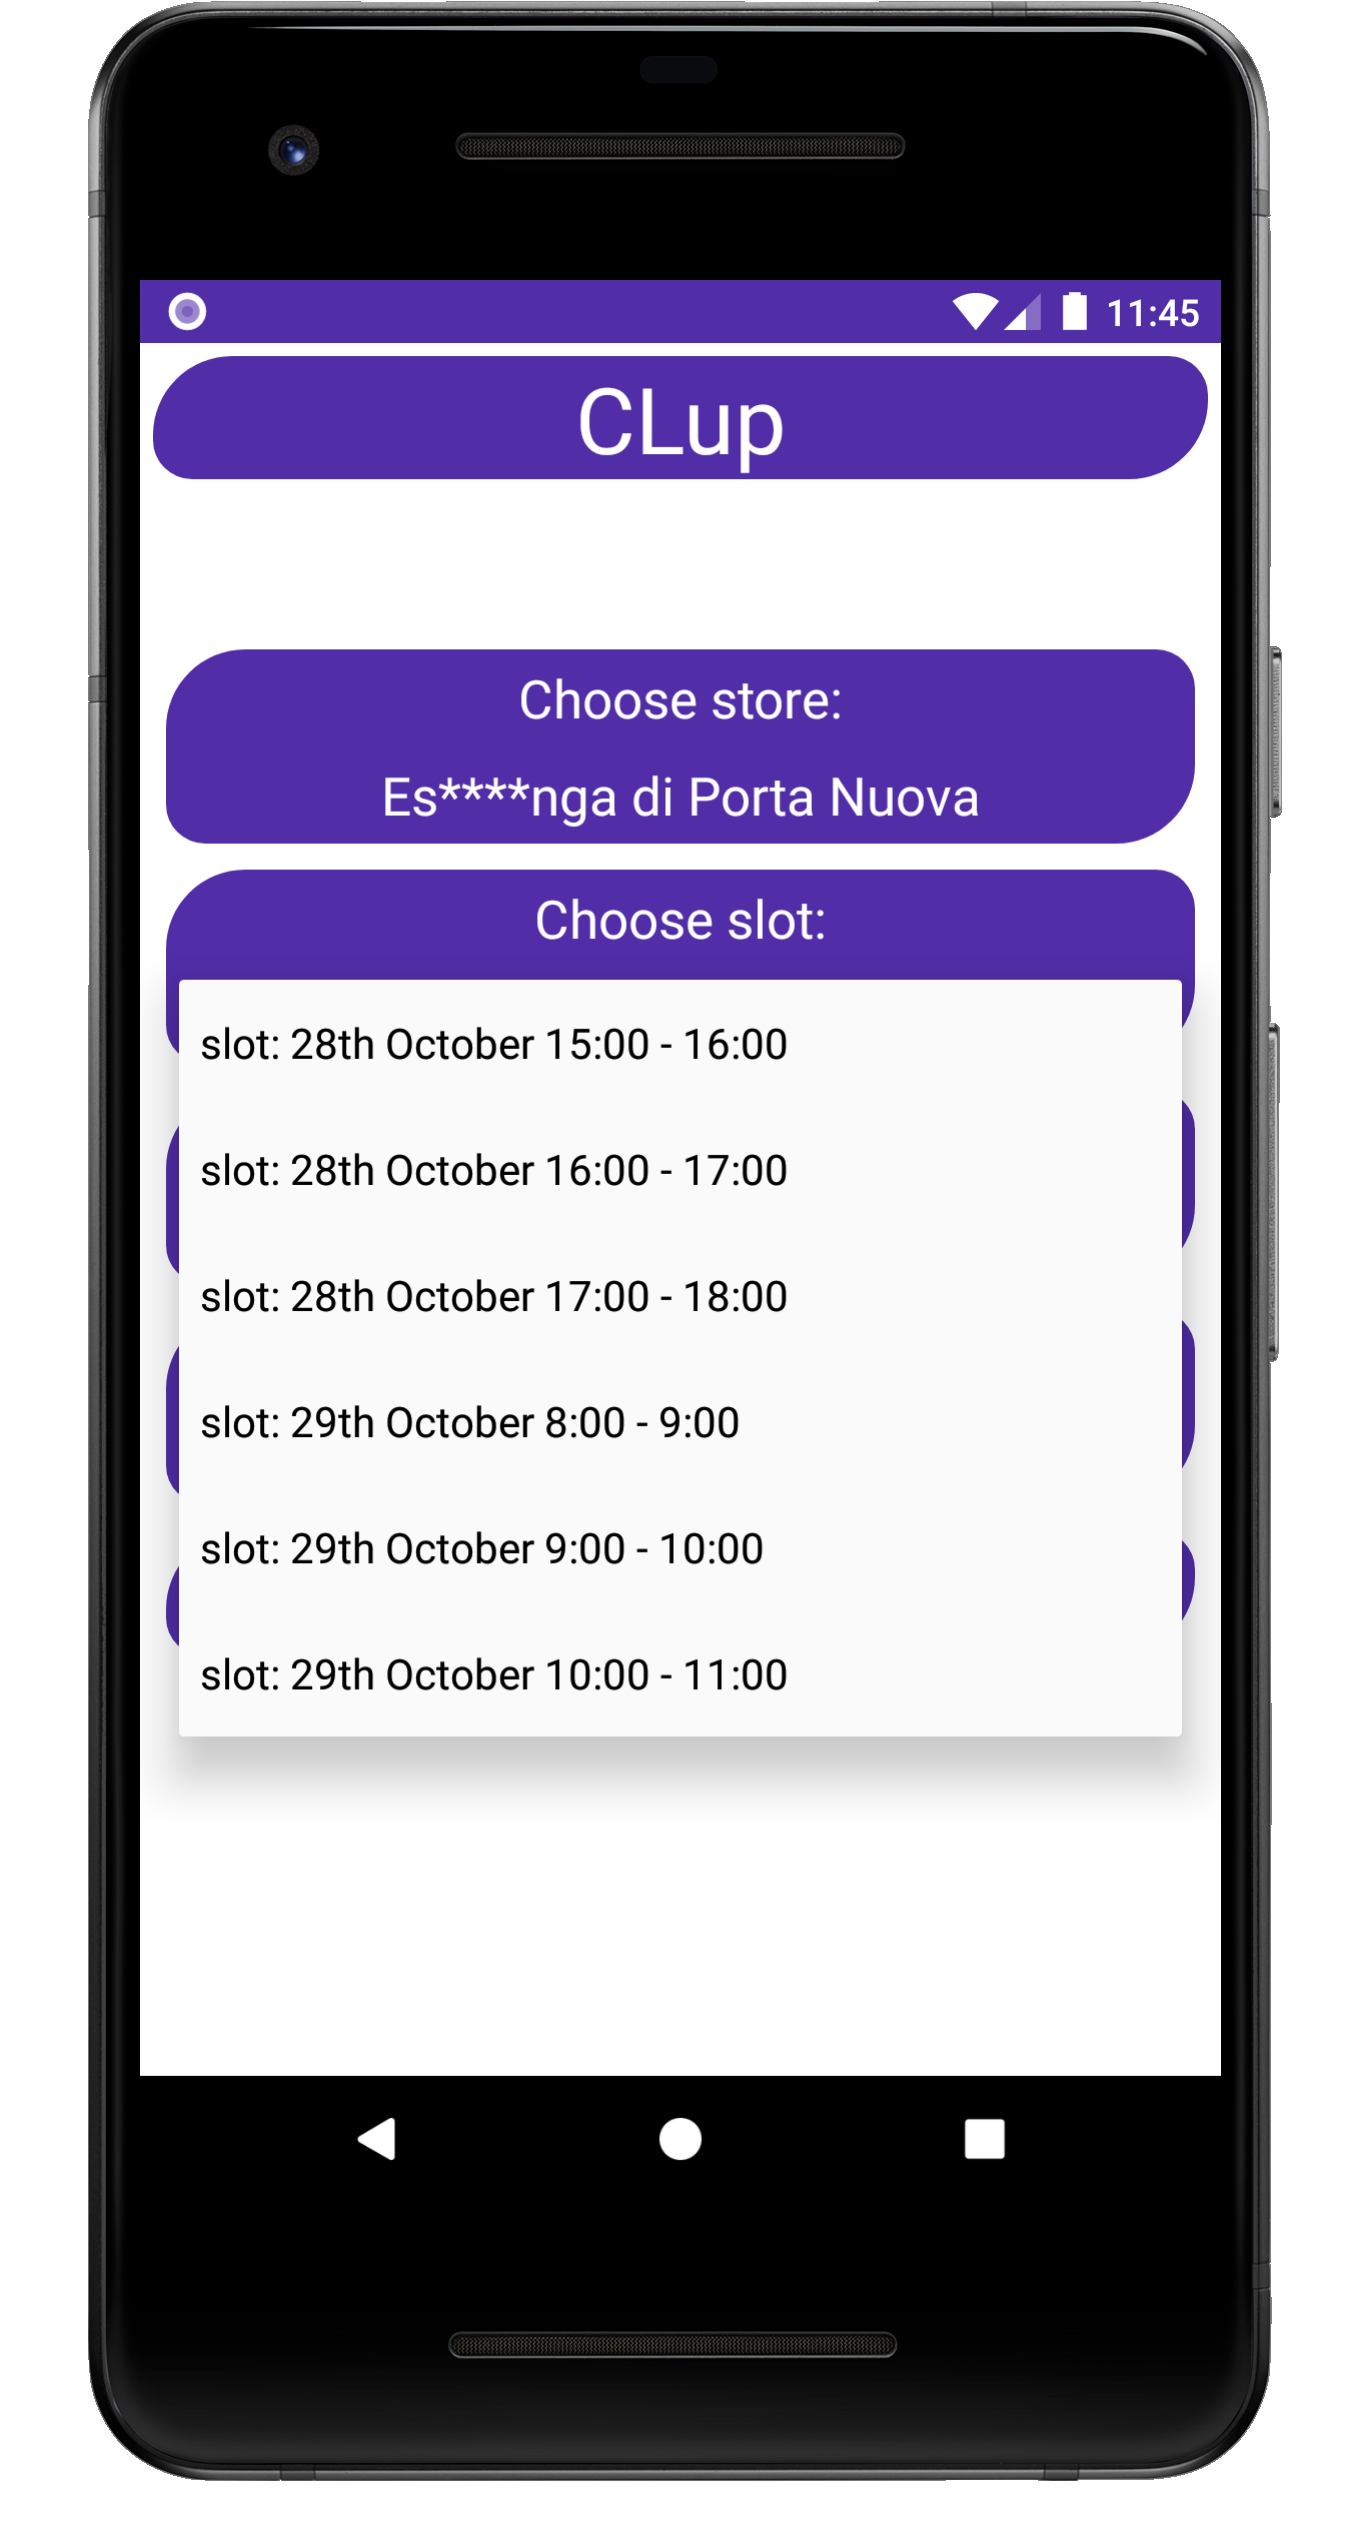
\includegraphics[width=0.4\textwidth]{images/booking_visit_02.png}}
	\caption{Example of Lining Up and Booking Visit pages.}
\end{figure}

\begin{figure}[H]
	\centering     %%% not \center
	\subfigure[Get Status page.]{\label{fig:a}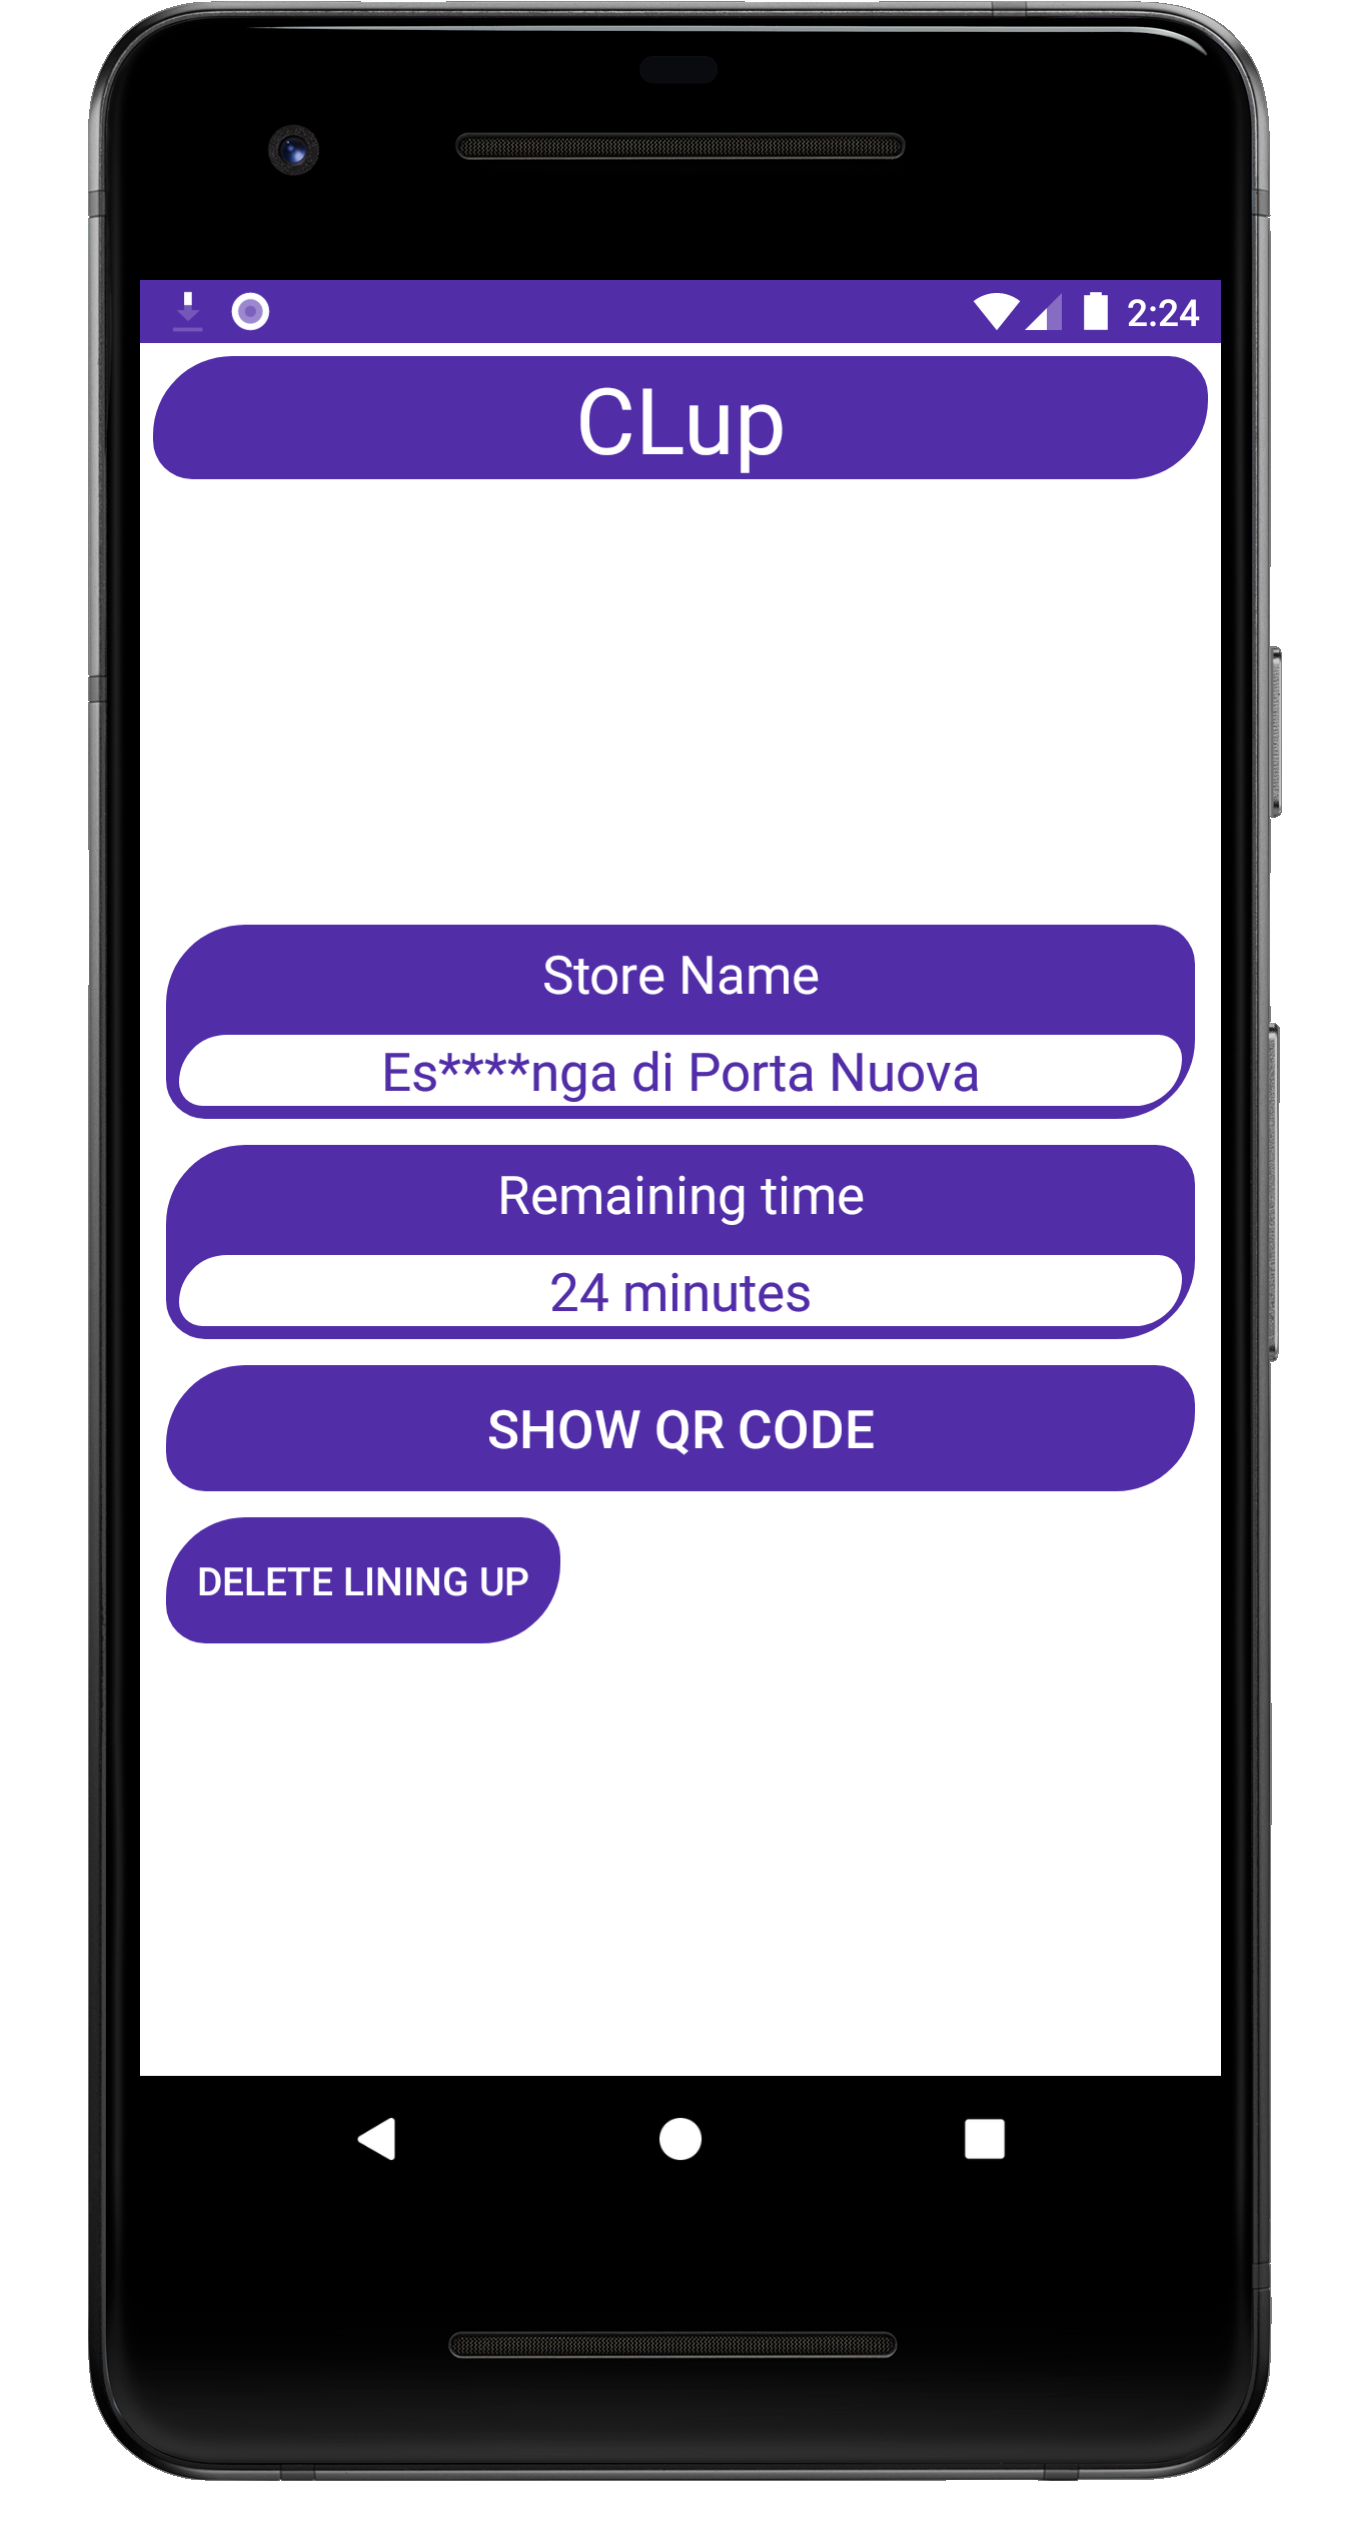
\includegraphics[width=0.4\textwidth]{images/get_status.png}}
	\subfigure[Show QR code page.]{\label{fig:b}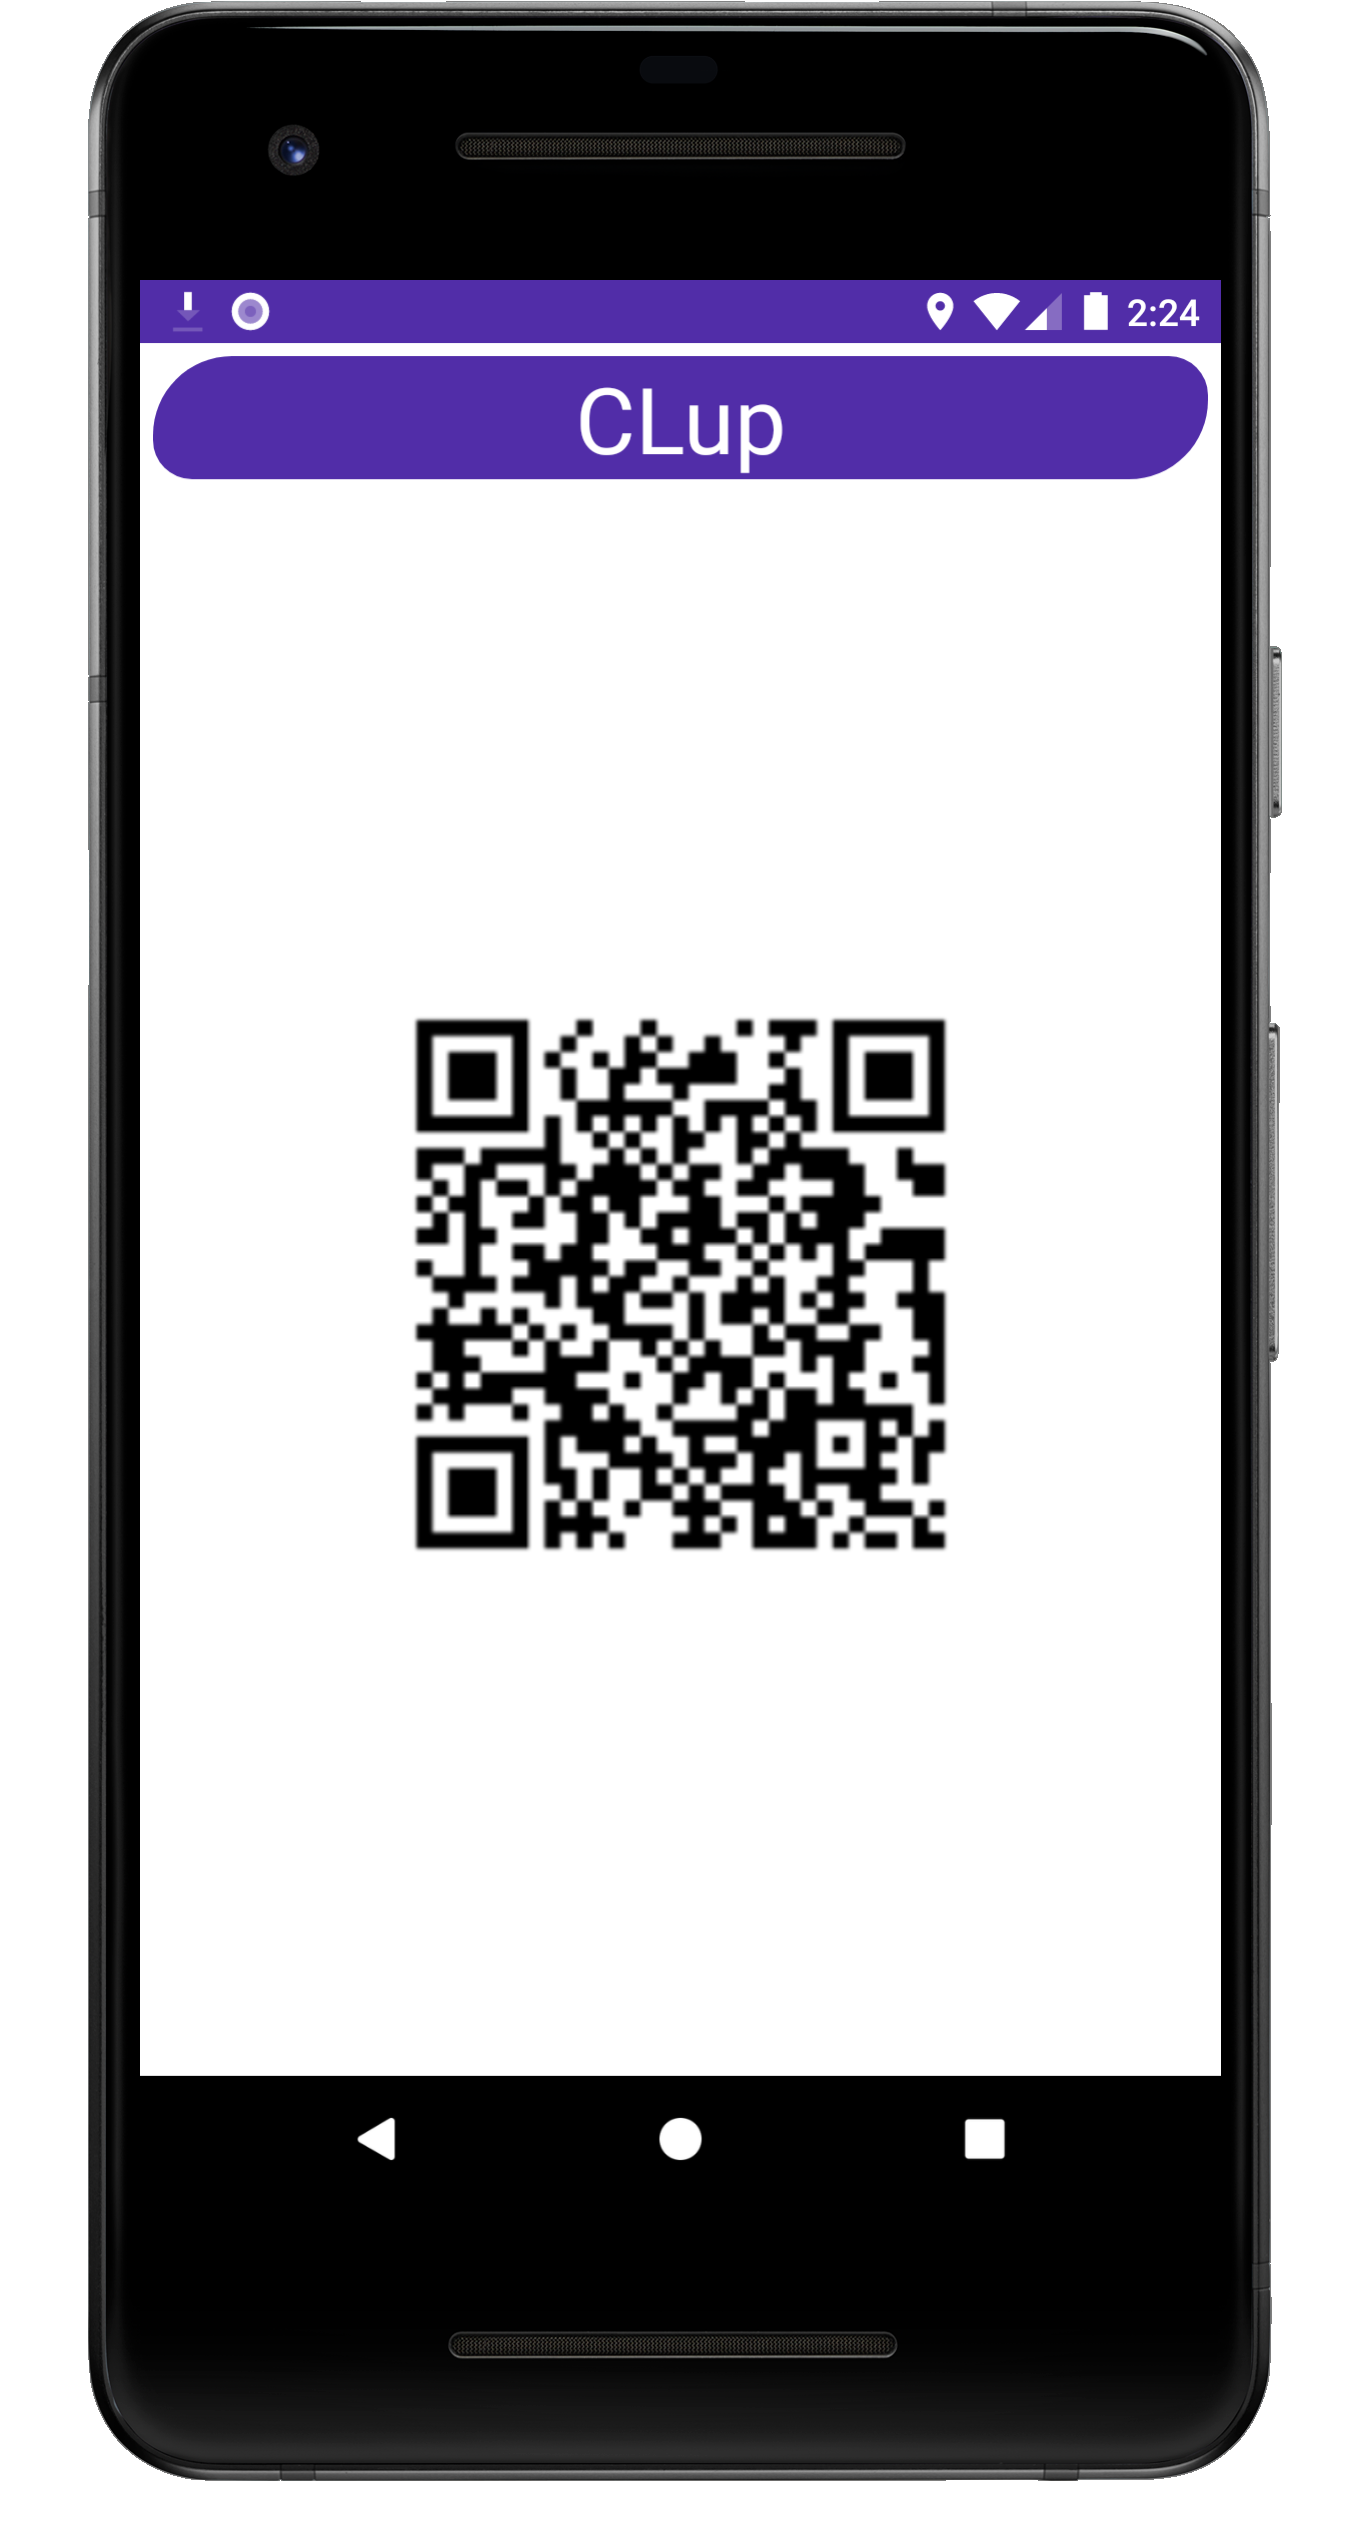
\includegraphics[width=0.4\textwidth]{images/show_qr_code.png}}
	\caption{Example of Get Status and Show QR code pages.}
\end{figure}


\subsection{Hardware Interfaces}
\subsection{Software interfaces}
\subsection{Communications Interfaces}

\section{Functional Requirements}

\subsection{Requirements}

Bla bla bla...

\begin{table}[H]
\centering
\begin{tabular}{| m{0.2\textwidth} | m{0.8\textwidth} |} 
	\hline
	\textbf{Goal} &
		\textbf{G1: Keep customers in safe condition w.r.t the \gls{dpcm} in force inside the store.} \\
		% requirements per gestire in flusso interno allo store, quindi planning
	\hline
	\textbf{Requirements} &
		\begin{itemize}
			\item {\textbf{[R]}}: The system has to
		\end{itemize} \\ 
	\hline
	\shortstack[l]{\textbf{Domain} \\ \textbf{Assumptions}} & 
		\begin{itemize}
			\item {\textbf{[D]}}: Customers follow the rules imposed by the \gls{dpcm} in force.
			\item {\textbf{[D]}}: Customers enter in the store only if the system, or the store manager, authorizes them.
			\item {\textbf{[D]}}: Customers don't stay in the shop longer than necessary.
			\item {\textbf{[D]}}: If customers booked a visit to the store and they specify the category of grocery, they won't buy other things.
			\item {\textbf{[D]}}: 
		\end{itemize} \\ 
	\hline
\end{tabular}
\end{table}

\begin{table}[H]
\centering
\begin{tabular}{| m{0.2\textwidth} | m{0.8\textwidth} |} 
	\hline
	\textbf{Goal} &
		\textbf{G2: Limit the physical line situation in the proximity of the store} \\
		% requirements per calcolare il tempo di arrivo, limitare il numero di prenotazioni ecc.
	\hline
	\textbf{Requirements} &
		\begin{itemize}
			\item {\textbf{[R]}}: The system has to estimate the residence time, of a customer, in the store.
			\item {\textbf{[R]}}: The system has to estimate the time needed to arrive, to the store, from the position of the customer.
			\item {\textbf{[R]}}: The system has to monitor the global position of the customers.
			\item {\textbf{[R]}}: The system has to limit the number of releasable QR code if imposed by the store manager.
		\end{itemize} \\ 
	\hline
	\shortstack[l]{\textbf{Domain} \\ \textbf{Assumptions}} & 
		\begin{itemize}
			\item {\textbf{[D]}}: Customers line up physically only if they have a valid (non expired) QR code.
			\item {\textbf{[D]}}: Customers go away from the store after they have done their shopping.
			\item {\textbf{[D]}}:
		\end{itemize} \\ 
	\hline
\end{tabular}
\end{table}

\begin{table}[H]
\centering
\begin{tabular}{| m{0.2\textwidth} | m{0.8\textwidth} |} 
	\hline
	\textbf{Goal} &
		\textbf{G3: Allow customers to line up from a remote device.} \\
		% requirements per l'app e il servizio di prenotazione (quality standard)
	\hline
	\textbf{Requirements} &
		\begin{itemize}
			\item {\textbf{[R]}}: Customers must be registered and logged in the application.
			\item {\textbf{[R]}}: The application has to implement the possibility to line up remotely.
			\item {\textbf{[R]}}: The application has to store locally the QR code.
			\item {\textbf{[R]}}: The application has to implement the possibility to delete a lining up operation.
			\item {\textbf{[R]}}:
		\end{itemize} \\ 
	\hline
	\shortstack[l]{\textbf{Domain} \\ \textbf{Assumptions}} & 
		\begin{itemize}
			\item {\textbf{[D]}}: The customers have a smartphone.
			\item {\textbf{[D]}}: The customers have installed the \gls{clup} application.
			\item {\textbf{[D]}}: The customers have a \gls{gps} module inside the smartphone.
			\item {\textbf{[D]}}: The customers allow the permissions requested by the application.
			\item {\textbf{[D]}}: The customers keep Internet connection active.
			\item {\textbf{[D]}}: The customers keep notification option active.
			\item {\textbf{[D]}}:
		\end{itemize} \\ 
	\hline
\end{tabular}
\end{table}

\begin{table}[H]
\centering
\begin{tabular}{| m{0.2\textwidth} | m{0.8\textwidth} |} 
	\hline
	\textbf{Goal} &
		\textbf{G4: Allow store manager to monitor entrances.} \\
		% requirements che implica l'implementazione nell'app dell'analisi del flusso, monito del tempistiche, previsioni ecc
		% + requirements per scan del QR code.
	\hline
	\textbf{Requirements} &
		\begin{itemize}
			\item {\textbf{[R]}}: The application has to show, to the store manager, analytical data concerning the influx of people to the store.
			\item {\textbf{[R]}}: The system has to allow, to the store manager, the possibility to limit the number of QR code released.
			\item {\textbf{[R]}}: The application shall allow the store manager to scan the QR codes.
			\item {\textbf{[R]}}:
		\end{itemize} \\ 
	\hline
	\shortstack[l]{\textbf{Domain} \\ \textbf{Assumptions}} & 
		\begin{itemize}
			\item {\textbf{[D]}}: There is always a store manager present in the store.
			\item {\textbf{[D]}}: The store manager has a digital device.
			\item {\textbf{[D]}}:
		\end{itemize} \\ 
	\hline
\end{tabular}
\end{table}

\begin{table}[H]
\centering
\begin{tabular}{| m{0.2\textwidth} | m{0.8\textwidth} |} 
	\hline
	\textbf{Goal} &
		\textbf{G5: Allow customers to line up from a physical spot.} \\
		% requirements per physical spot, caratteristiche, ecc
		% come influenza la gestione delle physical line situation?
	\hline
	\textbf{Requirements} &
		\begin{itemize}
			\item {\textbf{[R]}}:
		\end{itemize} \\ 
	\hline
	\shortstack[l]{\textbf{Domain} \\ \textbf{Assumptions}} & 
		\begin{itemize}
			\item {\textbf{[D]}}:
		\end{itemize} \\ 
	\hline
\end{tabular}
\end{table}

\begin{table}[H]
\centering
\begin{tabular}{| m{0.2\textwidth} | m{0.8\textwidth} |} 
	\hline
	\textbf{Goal} &
		\textbf{G6: Allow customers to book a visit from a remote device.} \\
		% requirements che implicano l'implementazione di una schermata nell'app per la prenotazione
	\hline
	\textbf{Requirements} &
		\begin{itemize}
			\item {\textbf{[R]}}:
		\end{itemize} \\ 
	\hline
	\shortstack[l]{\textbf{Domain} \\ \textbf{Assumptions}} & 
		\begin{itemize}
			\item {\textbf{[D]}}:
		\end{itemize} \\ 
	\hline
\end{tabular}
\end{table}

\begin{table}[H]
\centering
\begin{tabular}{| m{0.2\textwidth} | m{0.8\textwidth} |} 
	\hline
	\textbf{Goal} &
		\textbf{G7: Infer customers visits duration.} \\
		% requirements per il calcolo del tempo medio. Legato all'account dell'utente
	\hline
	\textbf{Requirements} &
		\begin{itemize}
			\item {\textbf{[R]}}:
		\end{itemize} \\ 
	\hline
	\shortstack[l]{\textbf{Domain} \\ \textbf{Assumptions}} & 
		\begin{itemize}
			\item {\textbf{[D]}}:
		\end{itemize} \\ 
	\hline
\end{tabular}
\end{table}


\subsection{Definition of Use Case Diagrams}

Bla bla bla...

\begin{figure}[H]
	\centering
	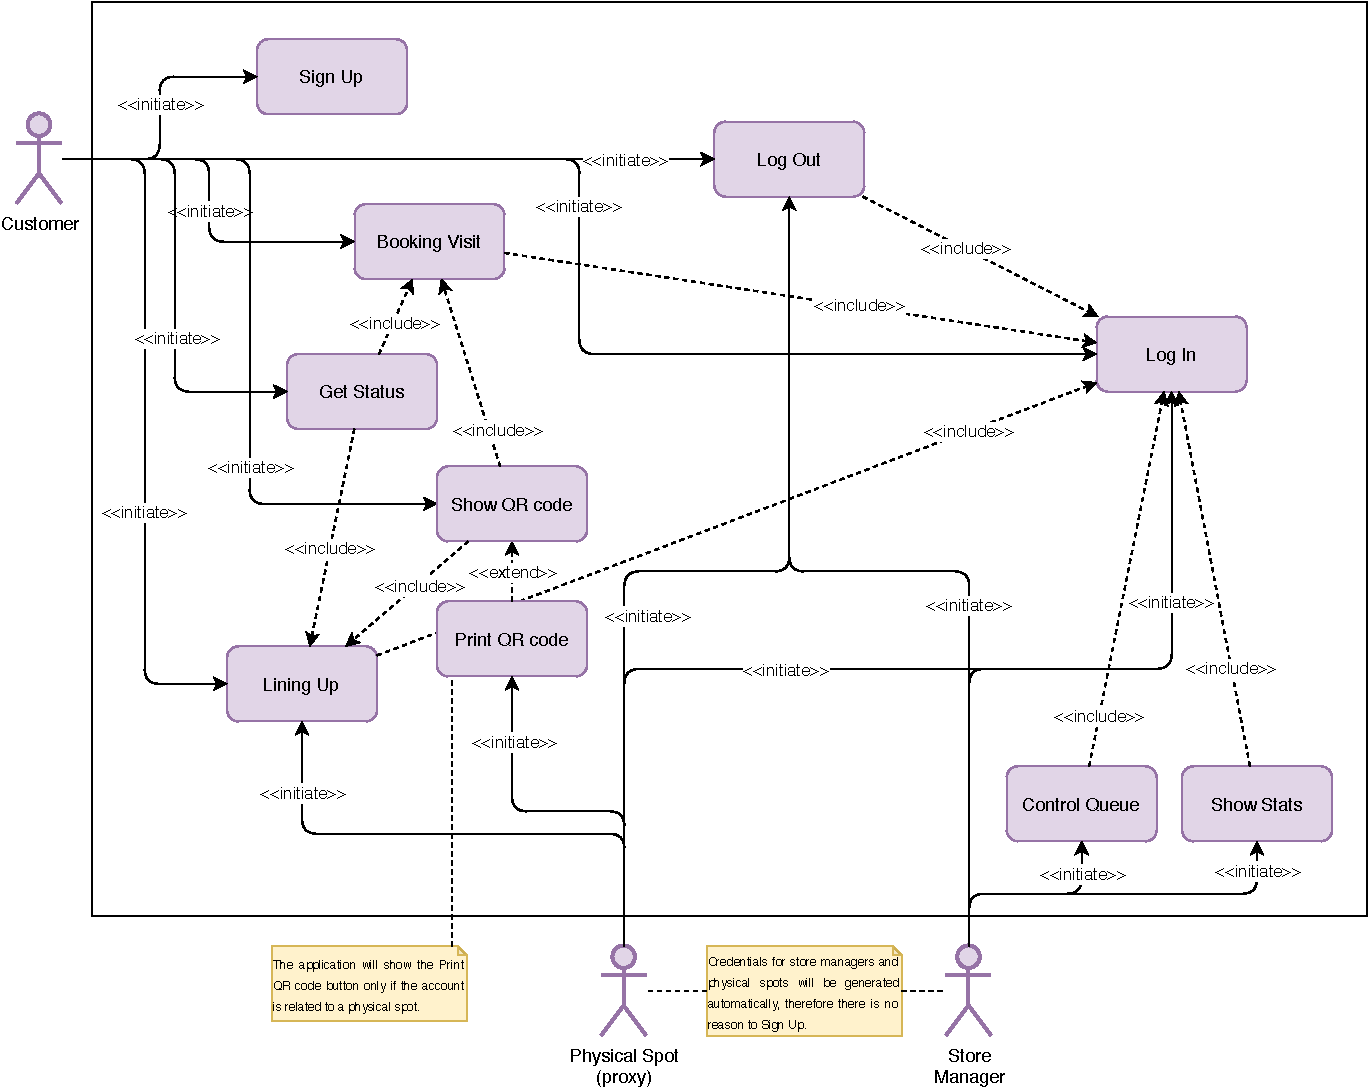
\includegraphics[width=1.0\textwidth]{images/use_cases_diagram.pdf}
	\caption{Use cases diagram.}
\end{figure}

\begin{table}[H]
\centering
\begin{tabular}{| m{0.3\textwidth} | m{0.7\textwidth} |} 
	\hline
	\textbf{Name} & Sign Up \\ 
	\hline
	\textbf{Actor} & Customer \\ 
	\hline
	\textbf{Entry Conditions} & Customer is on the Sign Up page. \\ 
	\hline
	\textbf{Event Flows} &
	\begin{itemize}
		\item Customer inserts the requested information in the form.
		\item Customer clicks on the Sign Up button.
	\end{itemize} \\ 
	\hline
	\textbf{Exit Conditions} & Sign Up completed successfully and customer is logged in, then the application shows the Home page. \\ 
	\hline
	\textbf{Exceptions} &
	\begin{itemize}
		\item Customer's username already in use.
		\item Empty form field.
		\item Policy agreement rejected.
		\item Lost Internet connection.
	\end{itemize} \\ 
	\hline
\end{tabular}
\caption{Use case: \textbf{Sign Up}.}
\label{tableSignUp}
\end{table}

\begin{table}[H]
\centering
\begin{tabular}{| m{0.3\textwidth} | m{0.7\textwidth} |} 
	\hline
	\textbf{Name} & Log In \\ 
	\hline
	\textbf{Actor} & Customer - Physical Spot - Store Manager \\ 
	\hline
	\textbf{Entry Conditions} & Actor is on the Log In page. \\ 
	\hline
	\textbf{Event Flows} &
	\begin{itemize}
	\item Actor inserts the requested information in the form.
	\item Actor clicks on the Log In button.
	\end{itemize} \\ 
	\hline
	\textbf{Exit Conditions} & Log In completed successfully and actor is redirected to the Home page. \\ 
	\hline
	\textbf{Exceptions} &
	\begin{itemize}
	\item Actor's username or password incorrect.
	\item Empty form field.
	\item Lost Internet connection.
	\end{itemize} \\ 
	\hline
\end{tabular}
\caption{Use case: \textbf{Log In}.}
\label{tableLogIn}
\end{table}

\begin{table}[H]
\centering
\begin{tabular}{| m{0.3\textwidth} | m{0.7\textwidth} |} 
	\hline
	\textbf{Name} & Log Out \\ 
	\hline
	\textbf{Actor} & Customer - Physical Spot - Store Manager \\ 
	\hline
	\textbf{Entry Conditions} & Actor is on the Log Out page. \\ 
	\hline
	\textbf{Event Flows} &
	\begin{itemize}
	\item Actor clicks on the Log Out button.
	\end{itemize} \\ 
	\hline
	\textbf{Exit Conditions} & Log Out completed successfully and actor is redirected to the Log In page. \\ 
	\hline
	\textbf{Exceptions} &
	\begin{itemize}
	\item Actor already logged out.
	\item Lost Internet connection.
	\end{itemize} \\ 
	\hline
\end{tabular}
\caption{Use case: \textbf{Log Out}.}
\label{tableLogOut}
\end{table}

\begin{table}[H]
\centering
\begin{tabular}{| m{0.3\textwidth} | m{0.7\textwidth} |} 
	\hline
	\textbf{Name} & Lining Up \\ 
	\hline
	\textbf{Actor} & Customer - Physical Spot \\ 
	\hline
	\textbf{Entry Conditions} & Actor is on the Home page. \\ 
	\hline
	\textbf{Event Flows} &
	\begin{itemize}
	\item Actor clicks on the Lining Up button.
	\item Actor inserts the requested data in the form.
	\item Actor clicks on the confirmation button.
	\end{itemize} \\ 
	\hline
	\textbf{Exit Conditions} & Lining Up completed successfully, the application returns the Status page. \\ 
	\hline
	\textbf{Exceptions} &
	\begin{itemize}
	\item Previous Lining Up action was not expired (only in case of remote customer).
	\item Previous Booking Visit action was not expired (only in case of remote customer).
	\item Actor wasn't logged.
	\item Lost Internet connection.
	\end{itemize} \\ 
	\hline
\end{tabular}
\caption{Use case: \textbf{Lining Up}.}
\label{tableLiningUp}
\end{table}

\begin{table}[H]
\centering
\begin{tabular}{| m{0.3\textwidth} | m{0.7\textwidth} |} 
	\hline
	\textbf{Name} & Booking Visit \\ 
	\hline
	\textbf{Actor} & Customer \\ 
	\hline
	\textbf{Entry Conditions} & Customer is on the Home page. \\ 
	\hline
	\textbf{Event Flows} &
	\begin{itemize}
	\item Customer clicks on the Booking Visit button.
	\item Customer fills the form with the requested data.
	\item Customer clicks on the Submit button.
	\end{itemize} \\ 
	\hline
	\textbf{Exit Conditions} & Booking Visit completed successfully and the application returns, to the customer, the Status page. \\ 
	\hline
	\textbf{Exceptions} &
	\begin{itemize}
	\item Previous Lining Up action was not expired.
	\item Previous Booking Visit action was not expired.
	\item Customer wasn't logged.
	\item Lost Internet connection.
	\end{itemize} \\ 
	\hline
\end{tabular}
\caption{Customer - use case: \textbf{Booking Visit}.}
\label{tableBookingVisit}
\end{table}

\begin{table}[H]
\centering
\begin{tabular}{| m{0.3\textwidth} | m{0.7\textwidth} |} 
	\hline
	\textbf{Name} & Show QR code - Print QR code \\ 
	\hline
	\textbf{Actor} & Customer - Physical Spot \\ 
	\hline
	\textbf{Entry Conditions} & Actor is on the Home page. \\ 
	\hline
	\textbf{Event Flows} &
	\begin{itemize}
	\item Actor clicks on the Show QR (Print QR) code button.
	\end{itemize} \\ 
	\hline
	\textbf{Exit Conditions} & The application shows (print) the QR code. \\ 
	\hline
	\textbf{Exceptions} &
	\begin{itemize}
	\item QR code wasn't saved on the application correctly (only in case of remote customer).
	\item No Lining Up, or Booking Visit, action previously performed (only in case of remote customer).
	\item Actor wasn't logged.
	\item Spot finished the paper.
	\item Spot finished the ink.
	\end{itemize} \\ 
	\hline
\end{tabular}
\caption{Use case: \textbf{Show QR code - Print QR code}.}
\label{tableShowQR}
\end{table}

\begin{table}[H]
\centering
\begin{tabular}{| m{0.3\textwidth} | m{0.7\textwidth} |} 
	\hline
	\textbf{Name} & Get Status \\ 
	\hline
	\textbf{Actor} & Customer \\ 
	\hline
	\textbf{Entry Conditions} & Customer is on the Home page. \\ 
	\hline
	\textbf{Event Flows} &
	\begin{itemize}
	\item Customer clicks on the Get Status button.
	\end{itemize} \\ 
	\hline
	\textbf{Exit Conditions} & The application returns the Get Status page showing information about the last Lining Up, or Booking Visit, operation. \\ 
	\hline
	\textbf{Exceptions} &
	\begin{itemize}
	\item No operation previously performed, therefore there is no data to show.
	\item Customer wasn't logged.
	\item Lost Internet connection.
	\end{itemize} \\ 
	\hline
\end{tabular}
\caption{Customer - use case: \textbf{Get Status}.}
\label{tableGetStatus}
\end{table}

\begin{table}[H]
\centering
\begin{tabular}{| m{0.3\textwidth} | m{0.7\textwidth} |} 
	\hline
	\textbf{Name} & Control Queue \\ 
	\hline
	\textbf{Actor} & Store Manager \\ 
	\hline
	\textbf{Entry Conditions} & Store Manager is on the Home page. \\ 
	\hline
	\textbf{Event Flows} &
	\begin{itemize}
	\item Store Manager clicks on the Control Queue button.
	\end{itemize} \\ 
	\hline
	\textbf{Exit Conditions} & The application returns the Control Queue page showing options to manage the queue. \\ 
	\hline
	\textbf{Exceptions} &
	\begin{itemize}
	\item Store Manager wasn't logged.
	\item Lost Internet connection.
	\end{itemize} \\ 
	\hline
\end{tabular}
\caption{Store Manager - use case: \textbf{Control Queue}.}
\label{tableGetStatus}
\end{table}

\begin{table}[H]
\centering
\begin{tabular}{| m{0.3\textwidth} | m{0.7\textwidth} |} 
	\hline
	\textbf{Name} & Show Stats \\ 
	\hline
	\textbf{Actor} & Store Manager \\ 
	\hline
	\textbf{Entry Conditions} & Store Manager is on the Home page. \\ 
	\hline
	\textbf{Event Flows} &
	\begin{itemize}
	\item Store Manager clicks on the Show Stats button.
	\end{itemize} \\ 
	\hline
	\textbf{Exit Conditions} & The application returns the Show Stats page showing information about the number of customers inside the store, the length of the queue and other information about the waiting time in queue. \\ 
	\hline
	\textbf{Exceptions} &
	\begin{itemize}
	\item Store Manager wasn't logged.
	\item Lost Internet connection.
	\end{itemize} \\ 
	\hline
\end{tabular}
\caption{Store Manager - use case: \textbf{Show Stats}.}
\label{tableGetStatus}
\end{table}


\subsection{Use Cases and Sequence/Activity Diagrams}

\begin{figure}[H]
	\centering
	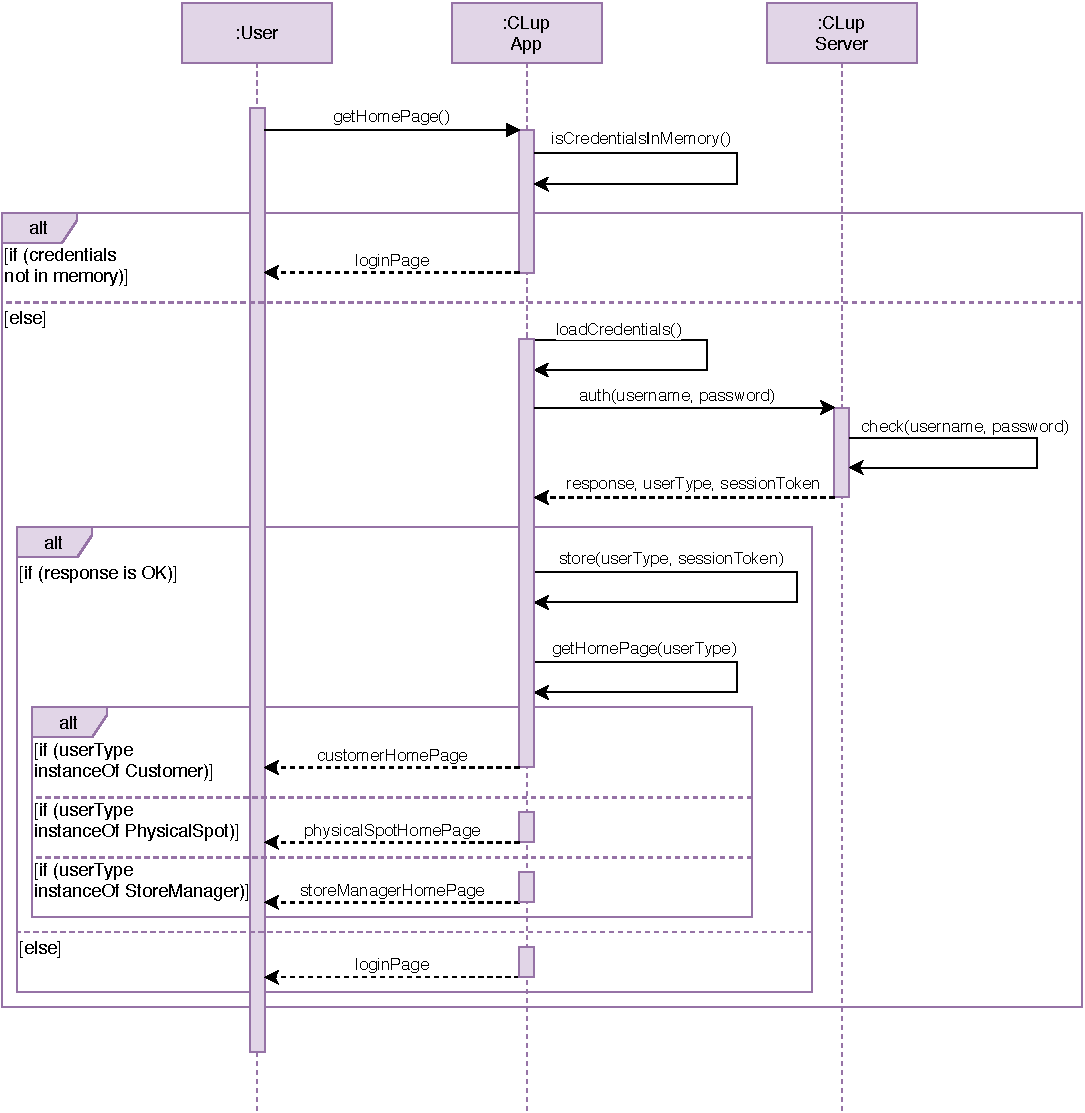
\includegraphics[width=1.0\textwidth]{images/getHomePage_sequence_diagram.pdf}
	\caption{Home page sequence diagram.}
\end{figure}

\begin{figure}[H]
	\centering
	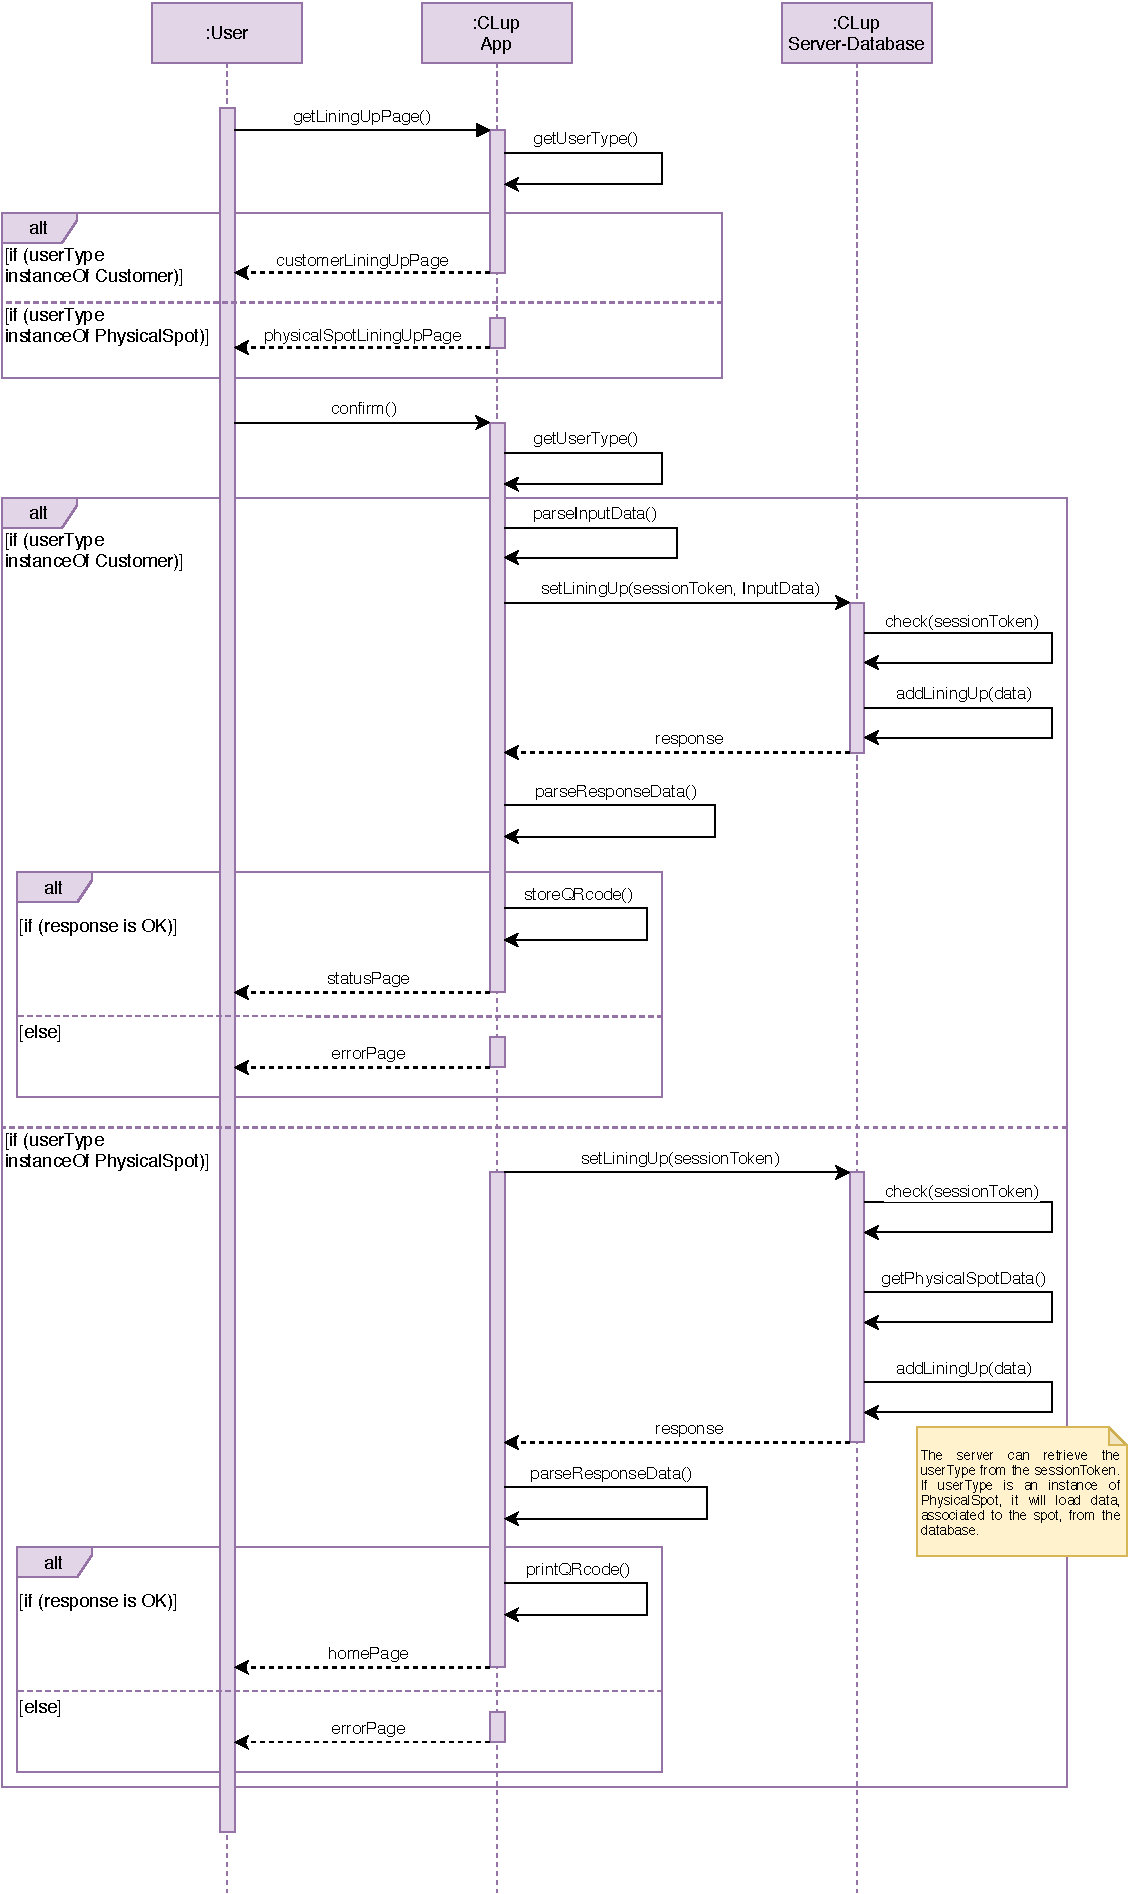
\includegraphics[width=1.0\textwidth]{images/liningUp_sequence_diagram.pdf}
	\caption{Lining Up sequence diagram.}
\end{figure}

\subsection{Mapping on Requirements}

\section{Performance Requirements}

\section{Design Constraints}

\subsection{Standard Compliance}
\subsection{Hardware limitations}
\subsection{Any Other Constraint}

\section{Software System Attributes}

\subsection{Reliability}
\subsection{Availability}
\subsection{Security}
\subsection{Maintainability}
\subsection{Portability}